\documentclass{article}

\usepackage[utf8]{inputenc}
\usepackage[T1]{fontenc}
\usepackage{geometry}
\usepackage{graphicx}   %ALLOWS INSERTING IMAGES (AND MAYBE SOME MORE STUFF) %
\usepackage{caption}
\usepackage{subcaption} %ALLOWS CAPTIONS FOR SUBFIGURES%
\usepackage{verbatim} % ALLOWS MULTILINE COMMENTS WITH \begin{comment} AND \end{comment} %
\usepackage{amsmath,amssymb} % PERMETTE L'USO DI SIMBOLI MATEMATICI "AVANZATI" COME 'MINORE O UGUALE' E ALTRI %
\usepackage{amstext}
\usepackage{enumitem} %PERMETTE L'USO DI ELENCHI NUMERATI
\usepackage[section]{placeins}
\usepackage[table]{xcolor} %tabelle colorate xdxdxd

\geometry{a4paper}
                        %Una riga vuota tra due scritte spazia di una riga anche sul pdf. Andare a capo una volta non provoca nulla nel pdf%
\usepackage[italian,english]{babel}
%\usepackage[french, italian]{babel} non funzione per motivi a me ignoti
\frenchspacing 

%%%  INTESTAZIONE  %%%

\title{Relazione dell'esperimento del reticolo olografico}
\author{Alessandro Matteo Rossi}
\date{20 gennaio 2021}



%%%  INIZIO DOCUMENTO  %%%

\begin{document}
\maketitle

%%%  ABSTRACT  %%%
\begingroup
\selectlanguage{english}
\begin{abstract}
    \centering
    L'obiettivo di questa esperienza domestica è usare un reticolo olografico di passo noto (chiamato "corto") per misurare le lunghezze d'onda emesse da una prima sorgente luminosa, il led di un puntatore laser e, attraverso queste, misurare il passo di un secondo reticolo (chiamato "lungo").
    L'esperimento si propone anche di misurare le lunghezze d'onda emesse da una seconda sorgente luminosa, una torcia a led, con entrambi i reticoli, per confrontarne i risultati.
    
    I risultati ottenuti sono stati:
    
    Passo del reticolo ignoto: \indent $d_{lungo} = 0,832 \pm 0,036 \; \mu m$

    \begin{table}[h]
        \centering
        \begin{tabular}[h]{||c|c|c|c||}
            \hline
            & \cellcolor{blue}$\lambda_{blue} [nm]$ & \cellcolor{green} $\lambda_{verde}[nm]$ & \cellcolor{red} $\lambda_{rosso}[nm]$\\
            \hline
            Puntatore & $442,6 \pm 7,4$ & $534,8 \pm 11,2$ & $654,0 \pm 21,7$\\
            \hline
            Torcia & $454,0 \pm 4,1$ & $ 558,1 \pm 8,8 $ & $ 686,5 \pm 10,5 $ \\
            \hline
        \end{tabular}
    \end{table}

\end{abstract}
\endgroup


%%%  INDICE  %%%%

\selectlanguage{italian}
\tableofcontents
\newpage

%%%  INTRODUZIONE TEORICA  %%%
%--------------------------------------------------------------------------------------------------------------------------------------------------------------------%
\section{Introduzione teorica}

La luce incidente su un reticolo di diffrazione subisce una diffrazione secondo l'equazione

\begin{equation}
    d(\sin\phi _m(\lambda)+\sin\theta) = m \lambda
    \label{general_equation}
\end{equation}

dove $d$ è il passo del reticolo, $m$ è l'ordine, $\phi_m$ è l'angolo di diffrazione all'm-esimo ordine, funzione della lunghezza d'onda $\lambda$ e $\theta$ è l'angolo di incidenza della luce sul reticolo.

\vspace{3mm}

Considerando che la luce utilizzata in ambiente domestico è divergente si hanno molteplici angoli di incidenza $\theta$. Per risolvere questa problematica, non potendo collimare il fascio luminoso con una lente, è conveniente distanziare di una quantità $z$ sufficientemente grande la sorgente luminosa e il reticolo per ottenere una condizione di raggi luminosi incidenti tra loro paralleli (Figura \ref{Schema_Diffrazione}). Ne discende che un sensore ottico posto dietro al reticolo ortogonale alla congiungente sorgente - reticolo vedrà i raggi come se provenissero dall'infinito, e pertanto con angolo di incidenza $\theta = 0$. Per questa esperienza si è scelto di usare come sensore ottico lo smartphone dello sperimentatore.

\begin{figure}[h]
    \centering
    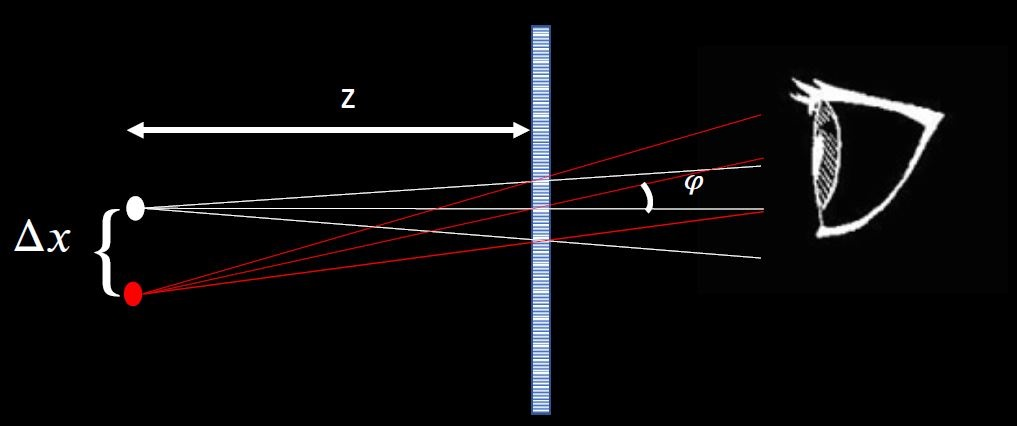
\includegraphics[width=0.55\linewidth]{Schema_Diffrazione.JPG}
    \caption{Disegno del sistema sorgente - reticolo - sensore. I raggi giungono paralleli al sensore, in questo caso un occhio. In questa trattazione l'angolo $\varphi$ viene chiamato $\phi$}
    \label{Schema_Diffrazione}
\end{figure}

In questa configurazione l'equazione (\ref{general_equation}) si riduce a 

\begin{equation}
    d \sin\phi_m(\lambda)=m\lambda
    \label{2nd_equation}
\end{equation}

Il sensore ottico vedrà attraverso il reticolo la sorgente e un'immagine diffratta, che per $z$ grande è assumibile come puntiforme.
Per considerazioni geometriche sulla Figura \ref{Schema_Diffrazione} 

\[\Delta x = z\tan\phi\]

Per il primo ordine ($m=1$) si può utilizzare l'approssimazione parassiale e assumere che 

\[z\tan\phi \approx z\sin\phi\]

e pertanto si ottiene 

\begin{equation}
    \Delta x = \frac{z \cdot \lambda}{d}
    \label{first_order_equation}
\end{equation}

dove $\Delta x$ è la distanza tra sorgente e immagine della lunghezza d'onda diffratta (complanare alla sorgente).

Se si osservasse il secondo ordine ($m=2$), l'angolo $\phi$ diventerebbe troppo grande per potere usare l'approssimazione parassiale e quindi bisognerebbe risalire al suo seno

\begin{equation}
    d\sin\left(\arctan\left(\frac{\Delta x}{z}\right)\right) = m\lambda
    \label{second_order_equation}
\end{equation}

%%%  PROGETTAZIONE DELL'ESPERIENZA  %%%
%--------------------------------------------------------------------------------------------------------------------------------------------------------------------%
\section{Progettazione dell'esperienza} \label{Progettazione}

L'esperienza è stata organizzata con gli strumenti a disposizione nell'abitazione. L'ambiente in cui si è svolta la misura è rappresentato in Figura \ref{ambiente}.

\begin{figure}[h!]
    \centering
    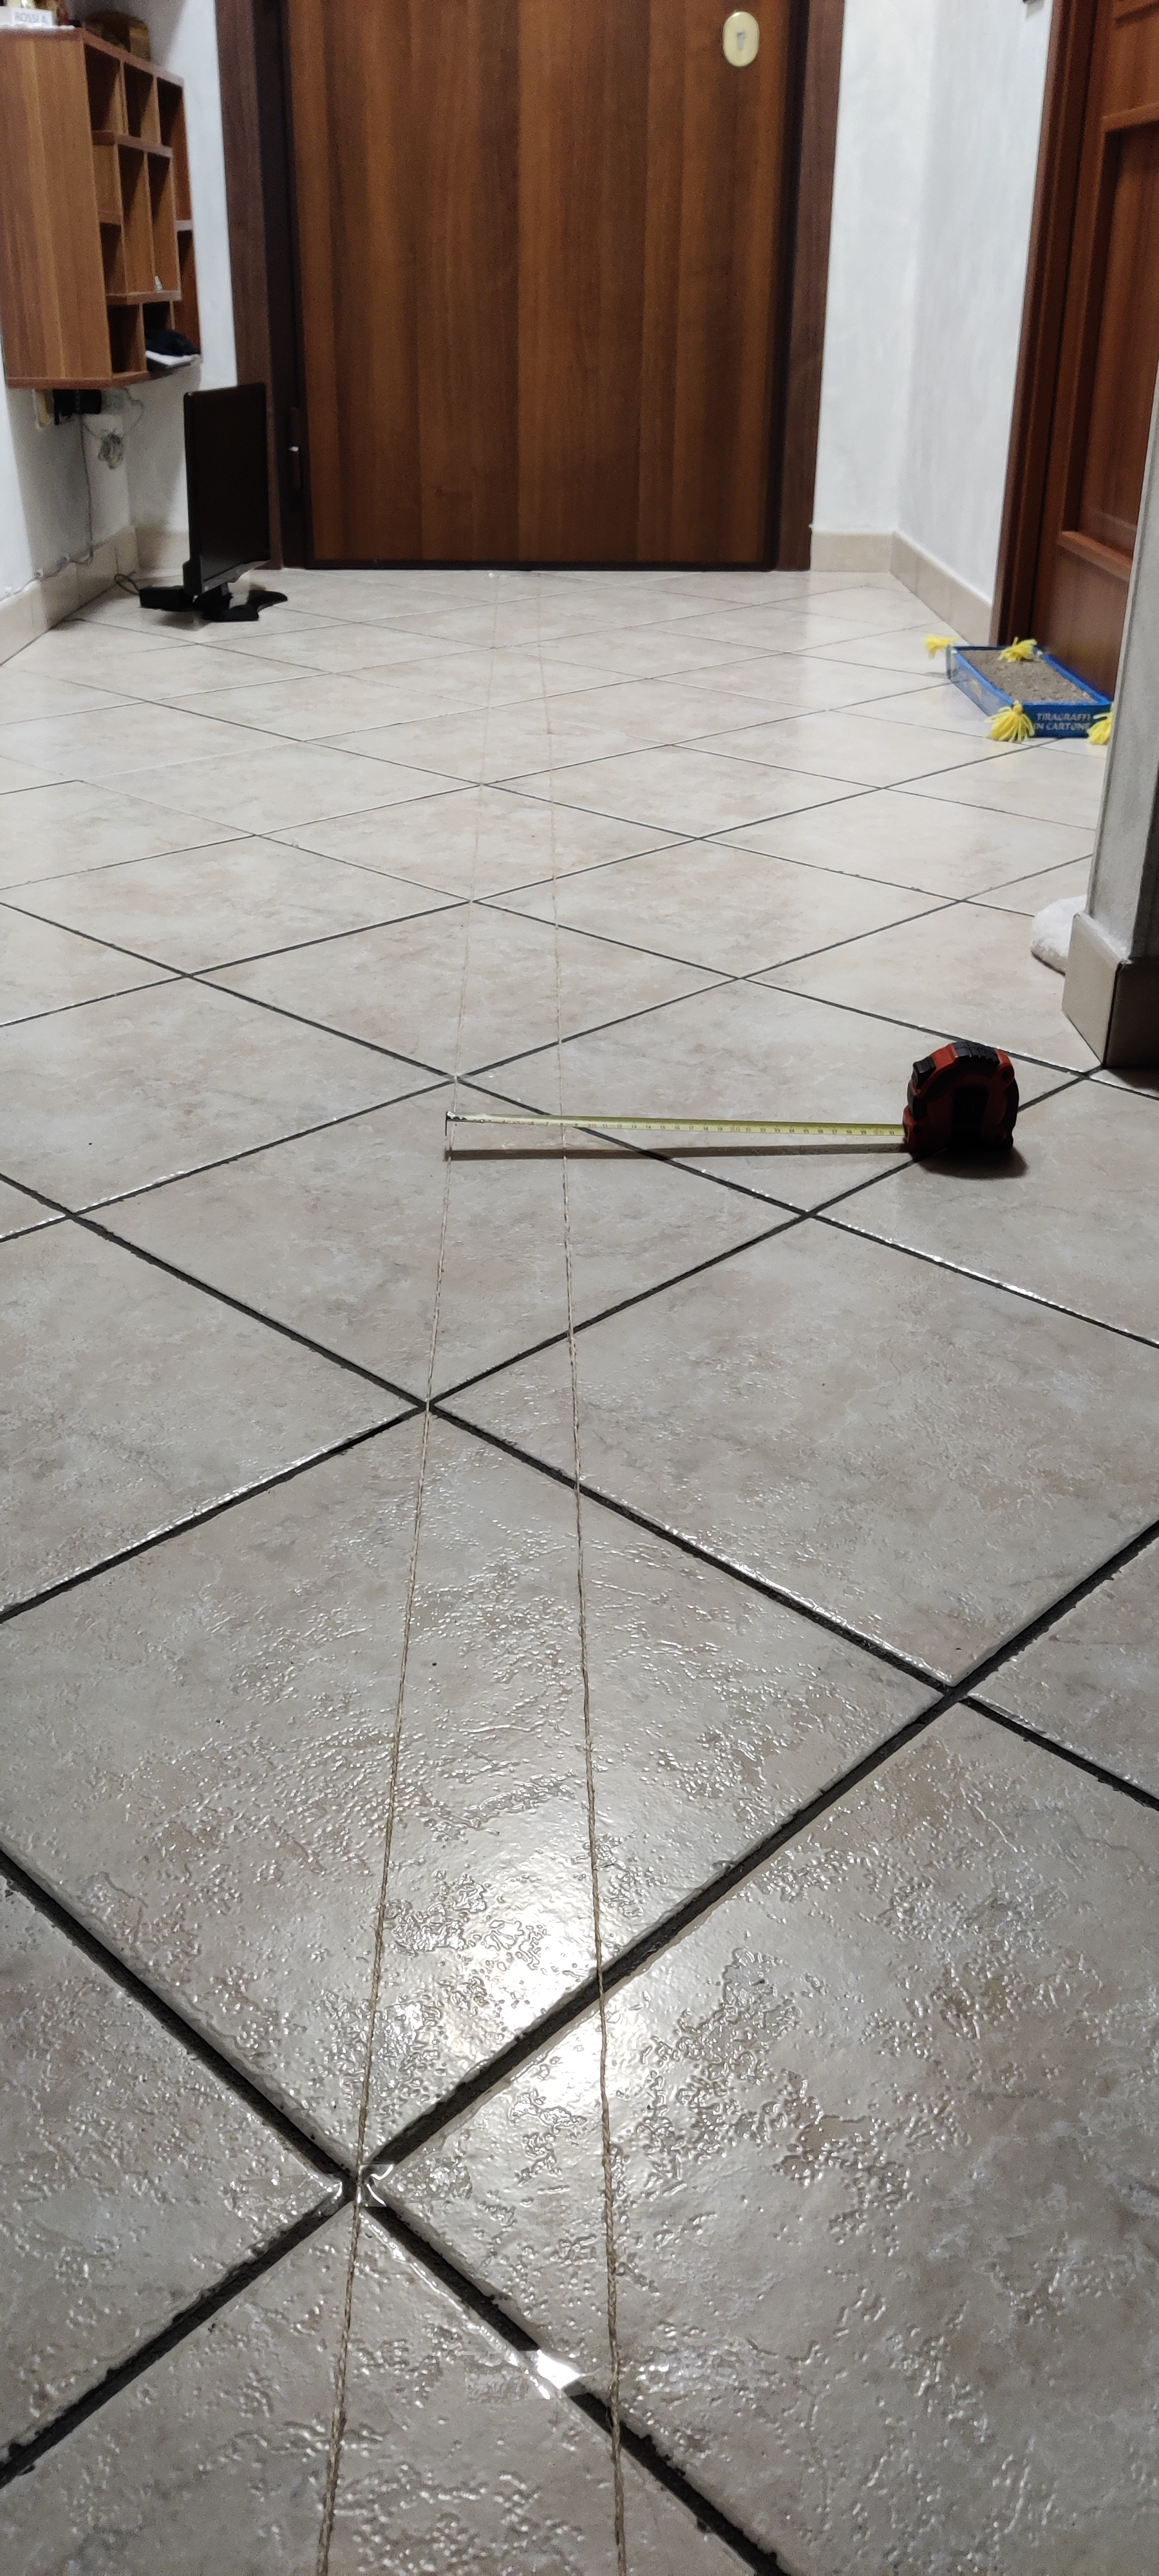
\includegraphics[width=0.2\linewidth]{Fili_Paralleli.jpg}
    \caption{Fotografia del laboratorio casalingo}
    \label{ambiente}
\end{figure}


Per prima cosa sono state scelte le sorgenti di luce. Si è optato per un puntatore laser con 2 led dedicati all'emissione di luce bianca, di cui uno oscurato con della pasta adesiva per diminuire l'intensità luminosa e facilitare quindi le misure, e una torcia a led, con intensità luminosa molto maggiore del puntatore. 

\begin{figure}[h!]
    \centering
    \begin{subfigure}[b]{0.4\linewidth}
        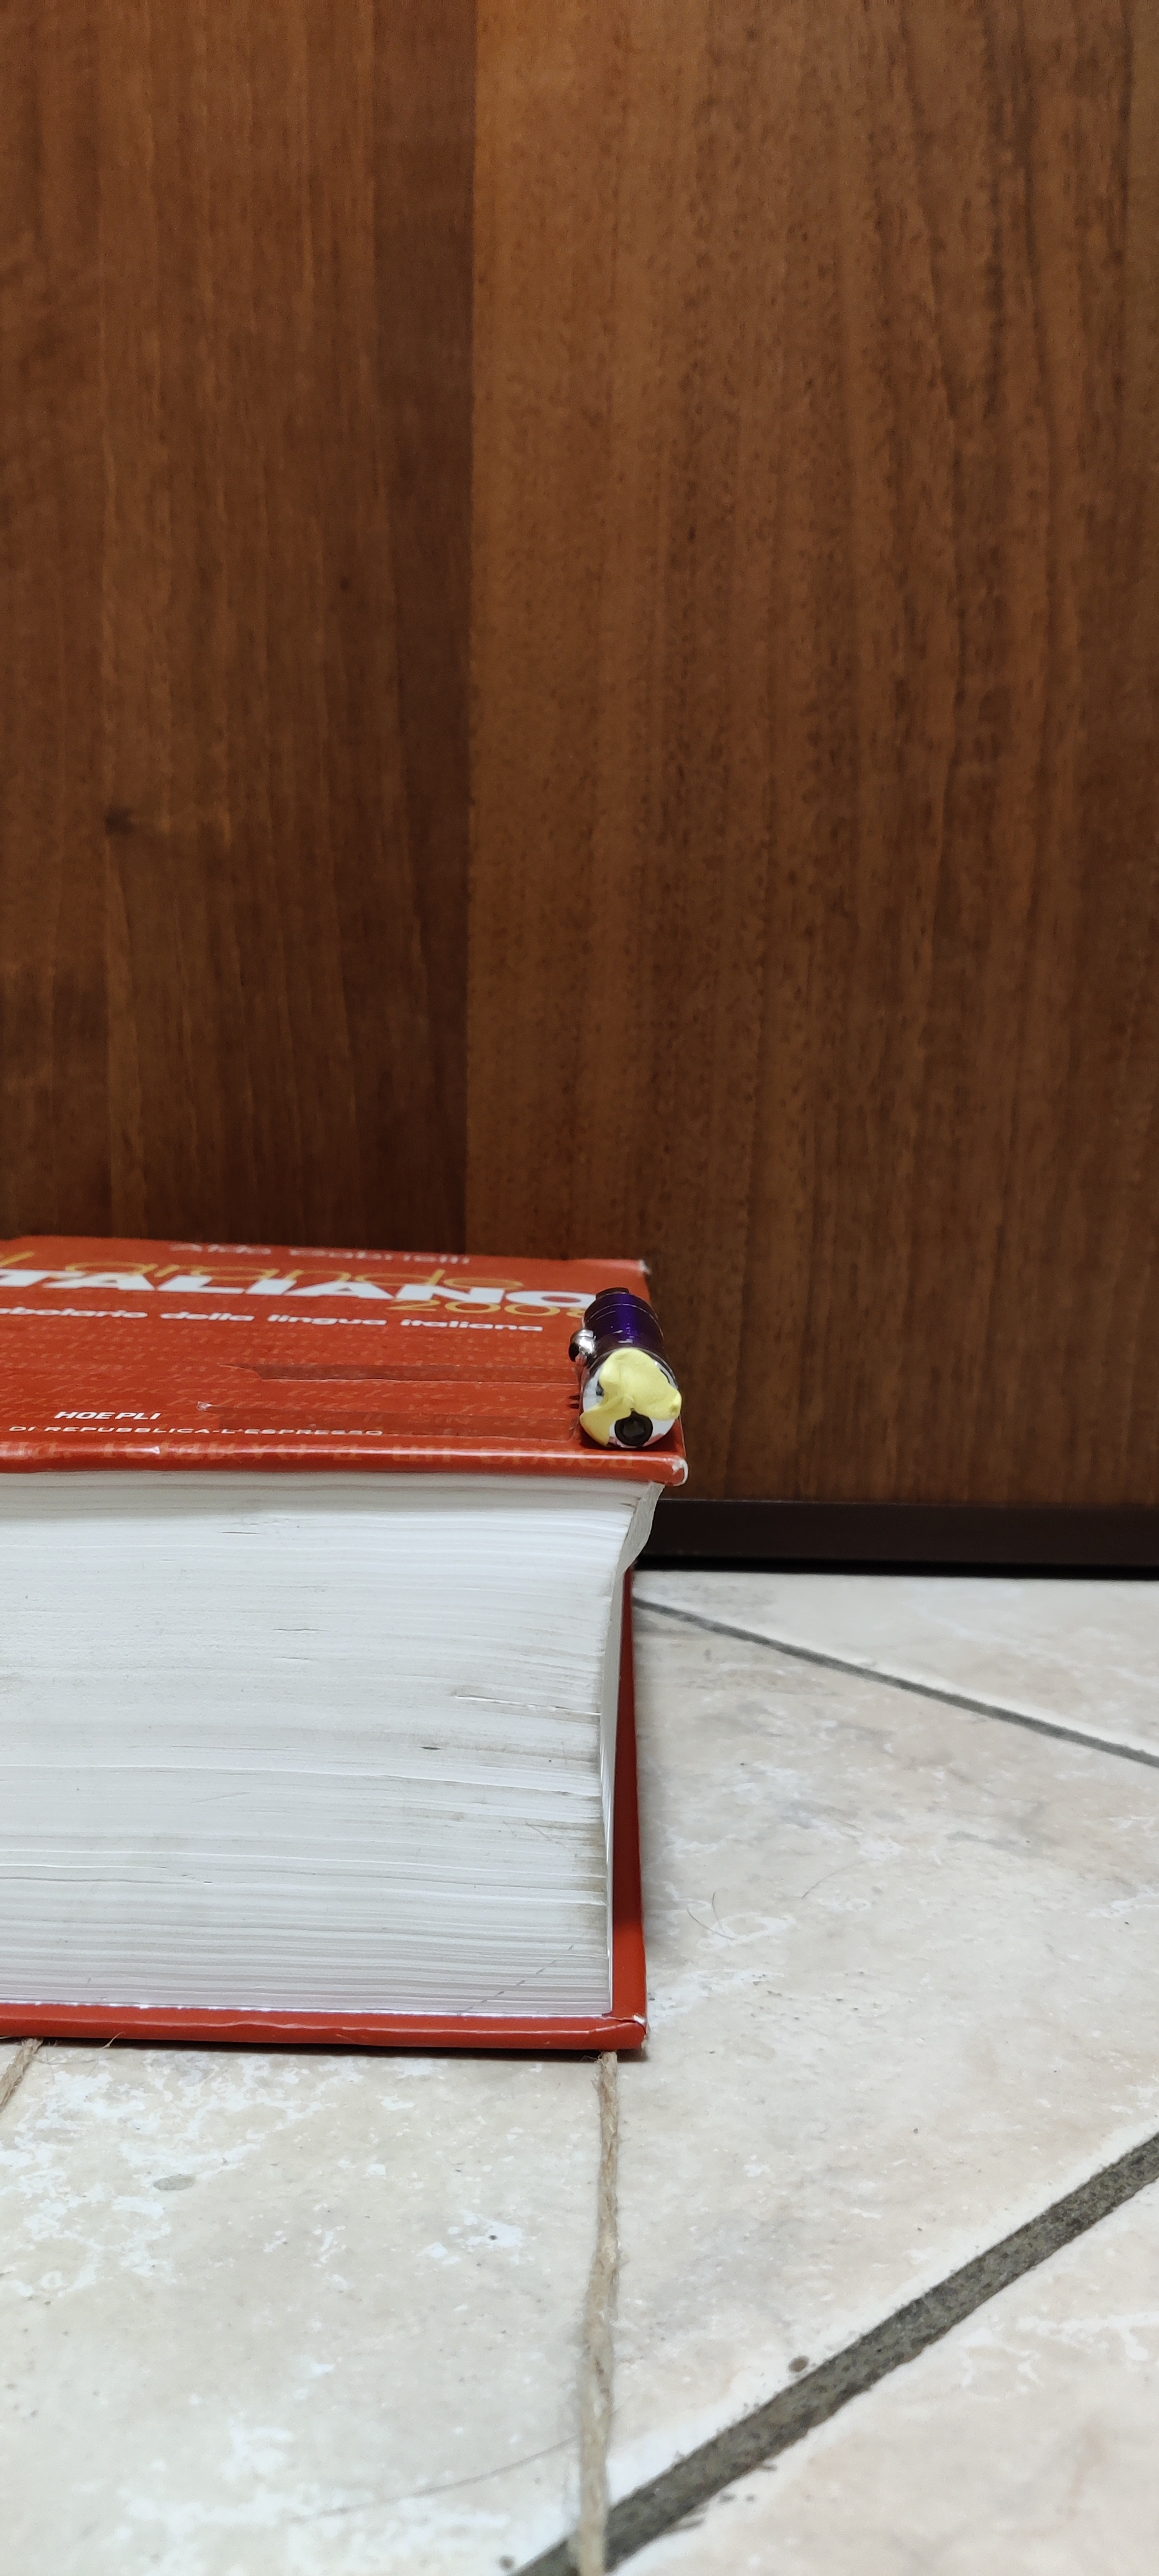
\includegraphics[width=\linewidth]{LedLungo0_Puntatore.jpg}
        \caption{Foto del puntatore laser, con un solo led lasciato scoperto}
    \end{subfigure}
    \begin{subfigure}[b]{0.32\linewidth}
        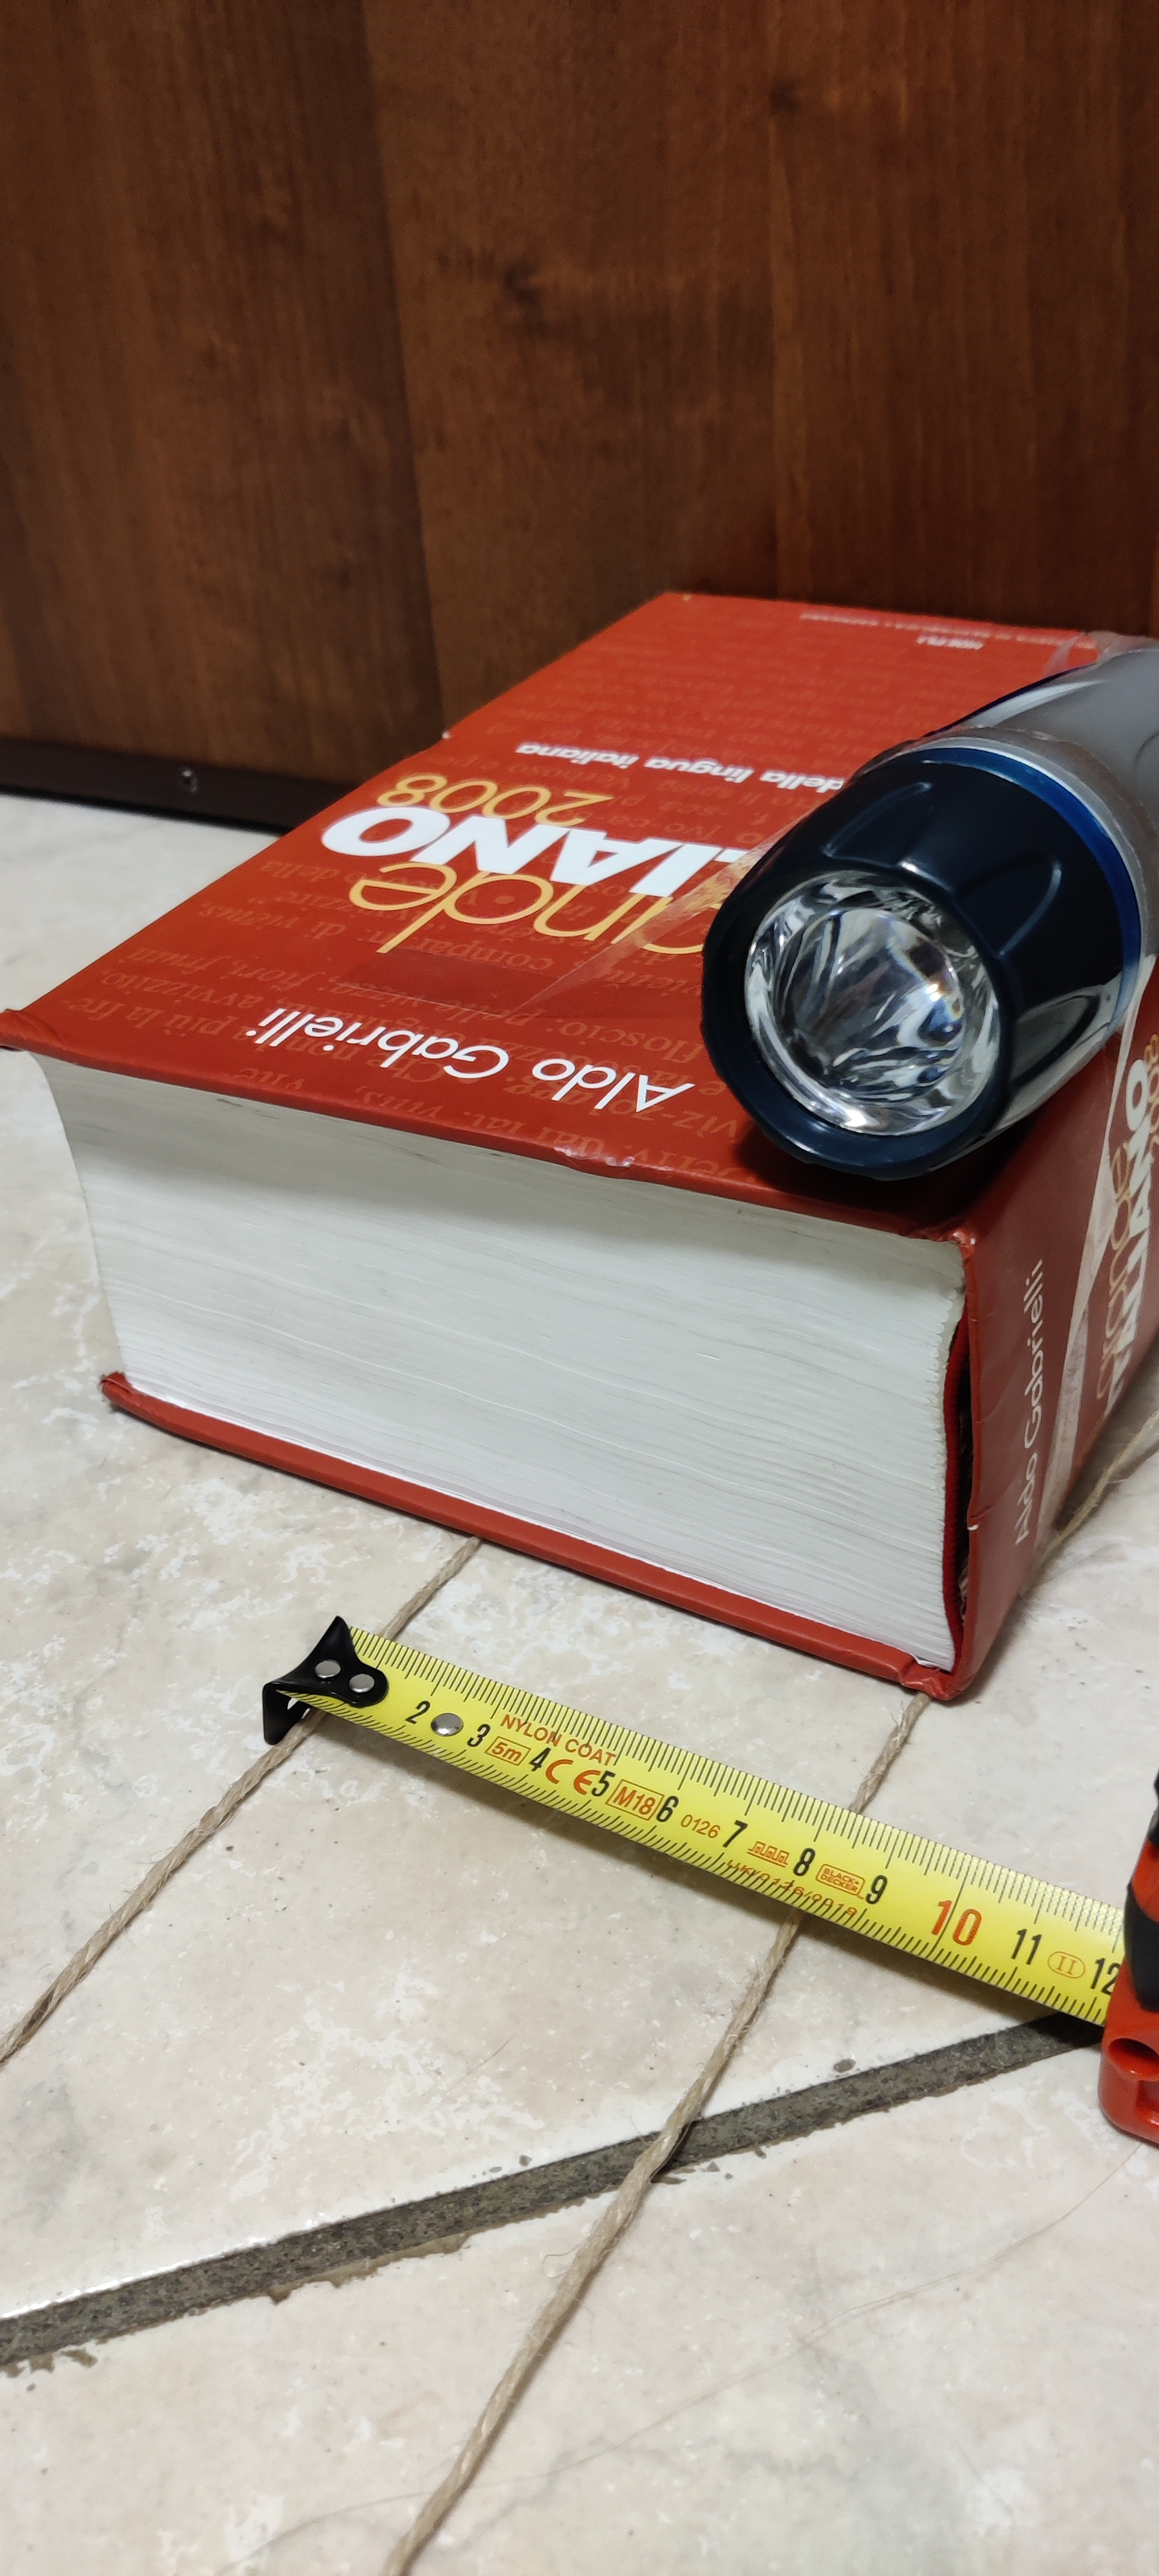
\includegraphics[width=\linewidth]{Torcia.jpg}
        \caption{Foto della torcia a led}
    \end{subfigure}
    \caption{Sorgenti di luce}
\end{figure}

Sfruttando le fughe del pavimento si è teso, e fissato con del nastro adesivo, uno spago lungo i vertici delle piastrelle perpendicolarmente alla porta (spago di sinistra in figura) per avere un riferimento che potesse collegare rettilineamente e ortogonalmente sorgente, reticolo e sensore ottico. Per maggiore simmetria rispetto ai muri si è teso un secondo spago (filo di destra), parallelo al primo, distante circa $8 \; cm$ . Quest'ultima scelta si è resa necessaria per evitare che il pavimento e il battiscopa, entrambi lucidi, producessero più riflessi di luce in uno dei due lati della fotografia. Ovviamente entrambi i fili sono stati posizionati con la massima precisione raggiungibile in ambiente domestico, pertanto verificando in più punti che fossero equidistanti ed evitando nella maniera più assoluta di calpestarli.

\vspace{3mm}

Per tutte le misure di lunghezza dell'esperienza è stato usato un metro a nastro sensibile al millimetro.

\vspace{3mm}

Fatto ciò, si è posizionato un tomo alto circa $8,5 \; cm$ con il bordo destro (rispetto alla figura) giacente sul filo di destra. Lungo questa retta verranno fissate con ulteriore nastro adesivo le sorgenti. 

\vspace{3mm}

Ultimata questa parte sono state oscurate porte e finestre, garantendo così il buio completo nel momento in cui fossero state spente le luci. 

\pagebreak

Per posizionare i reticoli sono stati usati:
\begin{enumerate}
    \item Un secondo tomo alto anch'esso $8,5 \; cm$ circa a cui fissare parallelamente al suolo il reticolo lungo, tenuto teso da uno stecchino di legno fissato sul lato lungo. Il reticolo si trovava circa alla stessa altezza dal suolo della sorgente.
    \item Due mollette da bucato identiche per il reticolo corto, per mantenerlo alla stessa altezza della sorgente dal pavimento, come mostrato in Figura \ref{impalcatura}
\end{enumerate}

\begin{figure}[h]
    \centering
    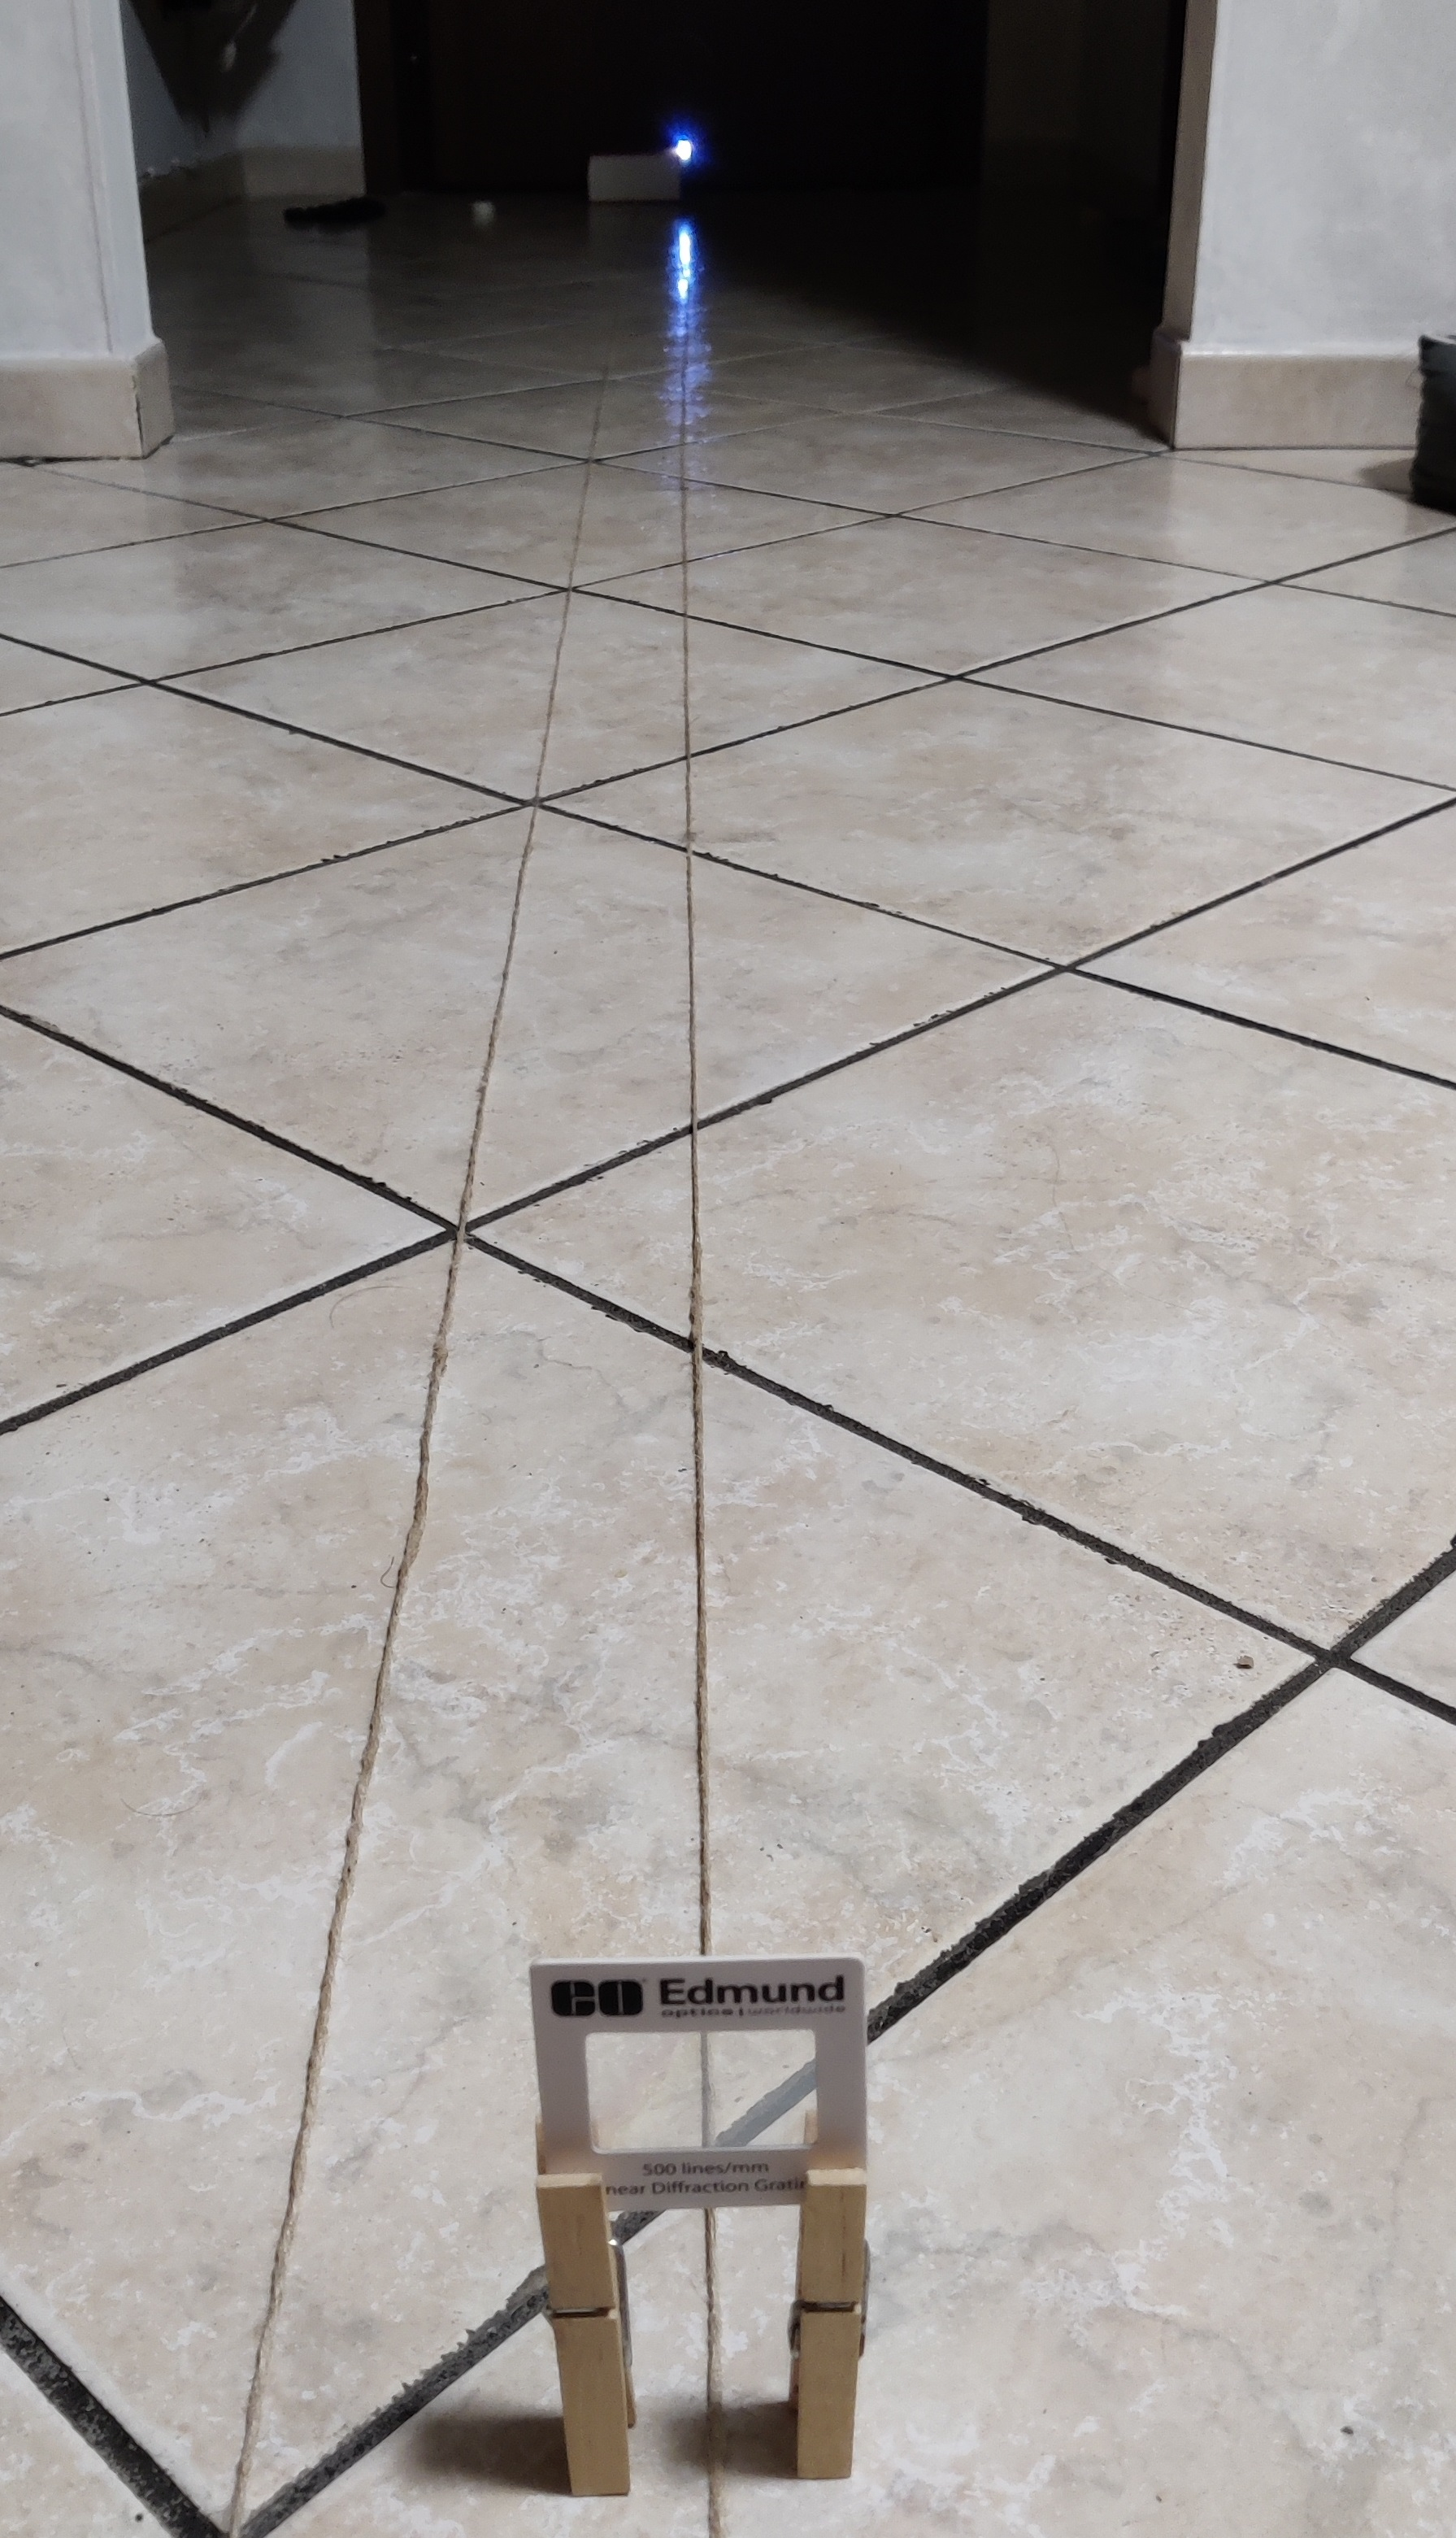
\includegraphics[width=0.2\linewidth]{LedCorto2_Impalcatura.jpg}
    \caption{Led corto sorretto da mollette per bucato alla stessa altezza della sorgente posta sul tomo}
    \label{impalcatura}
\end{figure}

Il posizionamento dello smartphone è stato effettuato con un ulteriore tomo che permettesse alla fotocamera di essere centrata sul reticolo e il più possibile ortogonale ad esso.

La distanza $z$ tra reticolo e sorgente si è mantenuta sempre intorno ai $4,43 \; m$. Per maggiore precisione è stata misurata più volte dopo ogni cambio di sorgente e/o reticolo. Si segnala che data la difficoltà di misurare distanze così lunghe con precisione, l'incertezza delle singole misure non è la sensibilità dello strumento o la deviazione standard ma $0,01 \; m$.
L'ortogonalità sorgente - reticolo - fotocamera è stata verificata e se necessario manualmente corretta ad ogni misura, osservando l'ombra che la sorgente produceva degli altri due elementi sul muro opposto ad essa e ruotando il reticolo sul proprio asse verticale di conseguenza.

\vspace{3mm}

Per analizzare le immagini raccolte e ricavare il valore di $\Delta x$ per potere risolvere le Equazioni (\ref{first_order_equation}) e (\ref{second_order_equation}), a seconda del'ordine, è stato utilizzato il software \textit{ImageJ} consigliato dai docenti. Per ogni misura è scattata almeno una foto a luce accesa e una a luce spenta: la prima per potere impostare la scala di misura sul software e la seconda per potere effettivamente raccogliere i valori di $\Delta x$ per i diversi colori diffratti.

\clearpage

%%%  PASSO DEL RETICOLO "LUNGO"  %%%
%--------------------------------------------------------------------------------------------------------------------------------------------------------------------%
\section{Passo del reticolo lungo}

La prima grandezza che si è voluta ricavare è il passo del reticolo lungo. Sono stati misurati i $\Delta x$ e quindi le lunghezze d'onda diffratte dal reticolo corto emesse dal puntatore attraverso l'Equazione (\ref{first_order_equation}), e conoscendo questi valori si sono potuti misurare i $\Delta x$ del reticolo lungo e ricavare il suo passo $d_{lungo}$.

\subsection{Misura \textrm{$\lambda_{puntatore}$}} \label{3.1}
Dopo avere posizionato la sorgente e il reticolo lungo come descritto in Sezione \ref{Progettazione} sono state raccolte 7 misure per la distanza sorgente-reticolo $z$ e altre 7 per la lunghezza del lato corto del vocabolario $L$ (complanare al punto di emissione di ambo le sorgenti). Quest'ultima sarà usata come lunghezza per definire la scala di misura su \textit{ImageJ} e rimarrà invariata per ogni misura. 

\begin{table}[h]
    \parbox{0.45\linewidth}{
        \centering
        \begin{tabular}{||c|c|c||}
            \hline
            \# & $z [m]$ & $\sigma_z [m]$\\
            \hline
            1 & 4,43 & 0,01 \\
            2 & 4,42 & 0,01 \\
            3 & 4,43 & 0,01 \\
            4 & 4,44 & 0,01 \\
            5 & 4,45 & 0,01 \\
            6 & 4,42 & 0,01 \\
            7 & 4,43 & 0,01 \\
            \hline
            $z_{best}$ & 4,43 & 0,01 \\
            \hline
        \end{tabular}
        \caption{Misura di $z$}
% \end{table}
    }
\parbox{0.45\linewidth}{
% \begin{table}
    \centering
    \begin{tabular}{||c|c|c||}
        \hline
        \# & $L [m]$ & $\sigma_L [m]$ \\
        \hline
        1 & 0,166 & 0,001 \\
        2 & 0,166 & 0,001 \\
        3 & 0,167 & 0,001 \\
        4 & 0,168 & 0,001 \\
        5 & 0,165 & 0,001 \\
        6 & 0,166 & 0,001 \\
        7 & 0,165 & 0,001 \\
        \hline
        $L_{best}$ & 4,43 & 0,001 \\
        \hline
    \end{tabular}
    \caption{Misura della lunghezza del lato corto del vocabolario $L$}
}    
\end{table}

\begin{figure}[h]
    \centering
    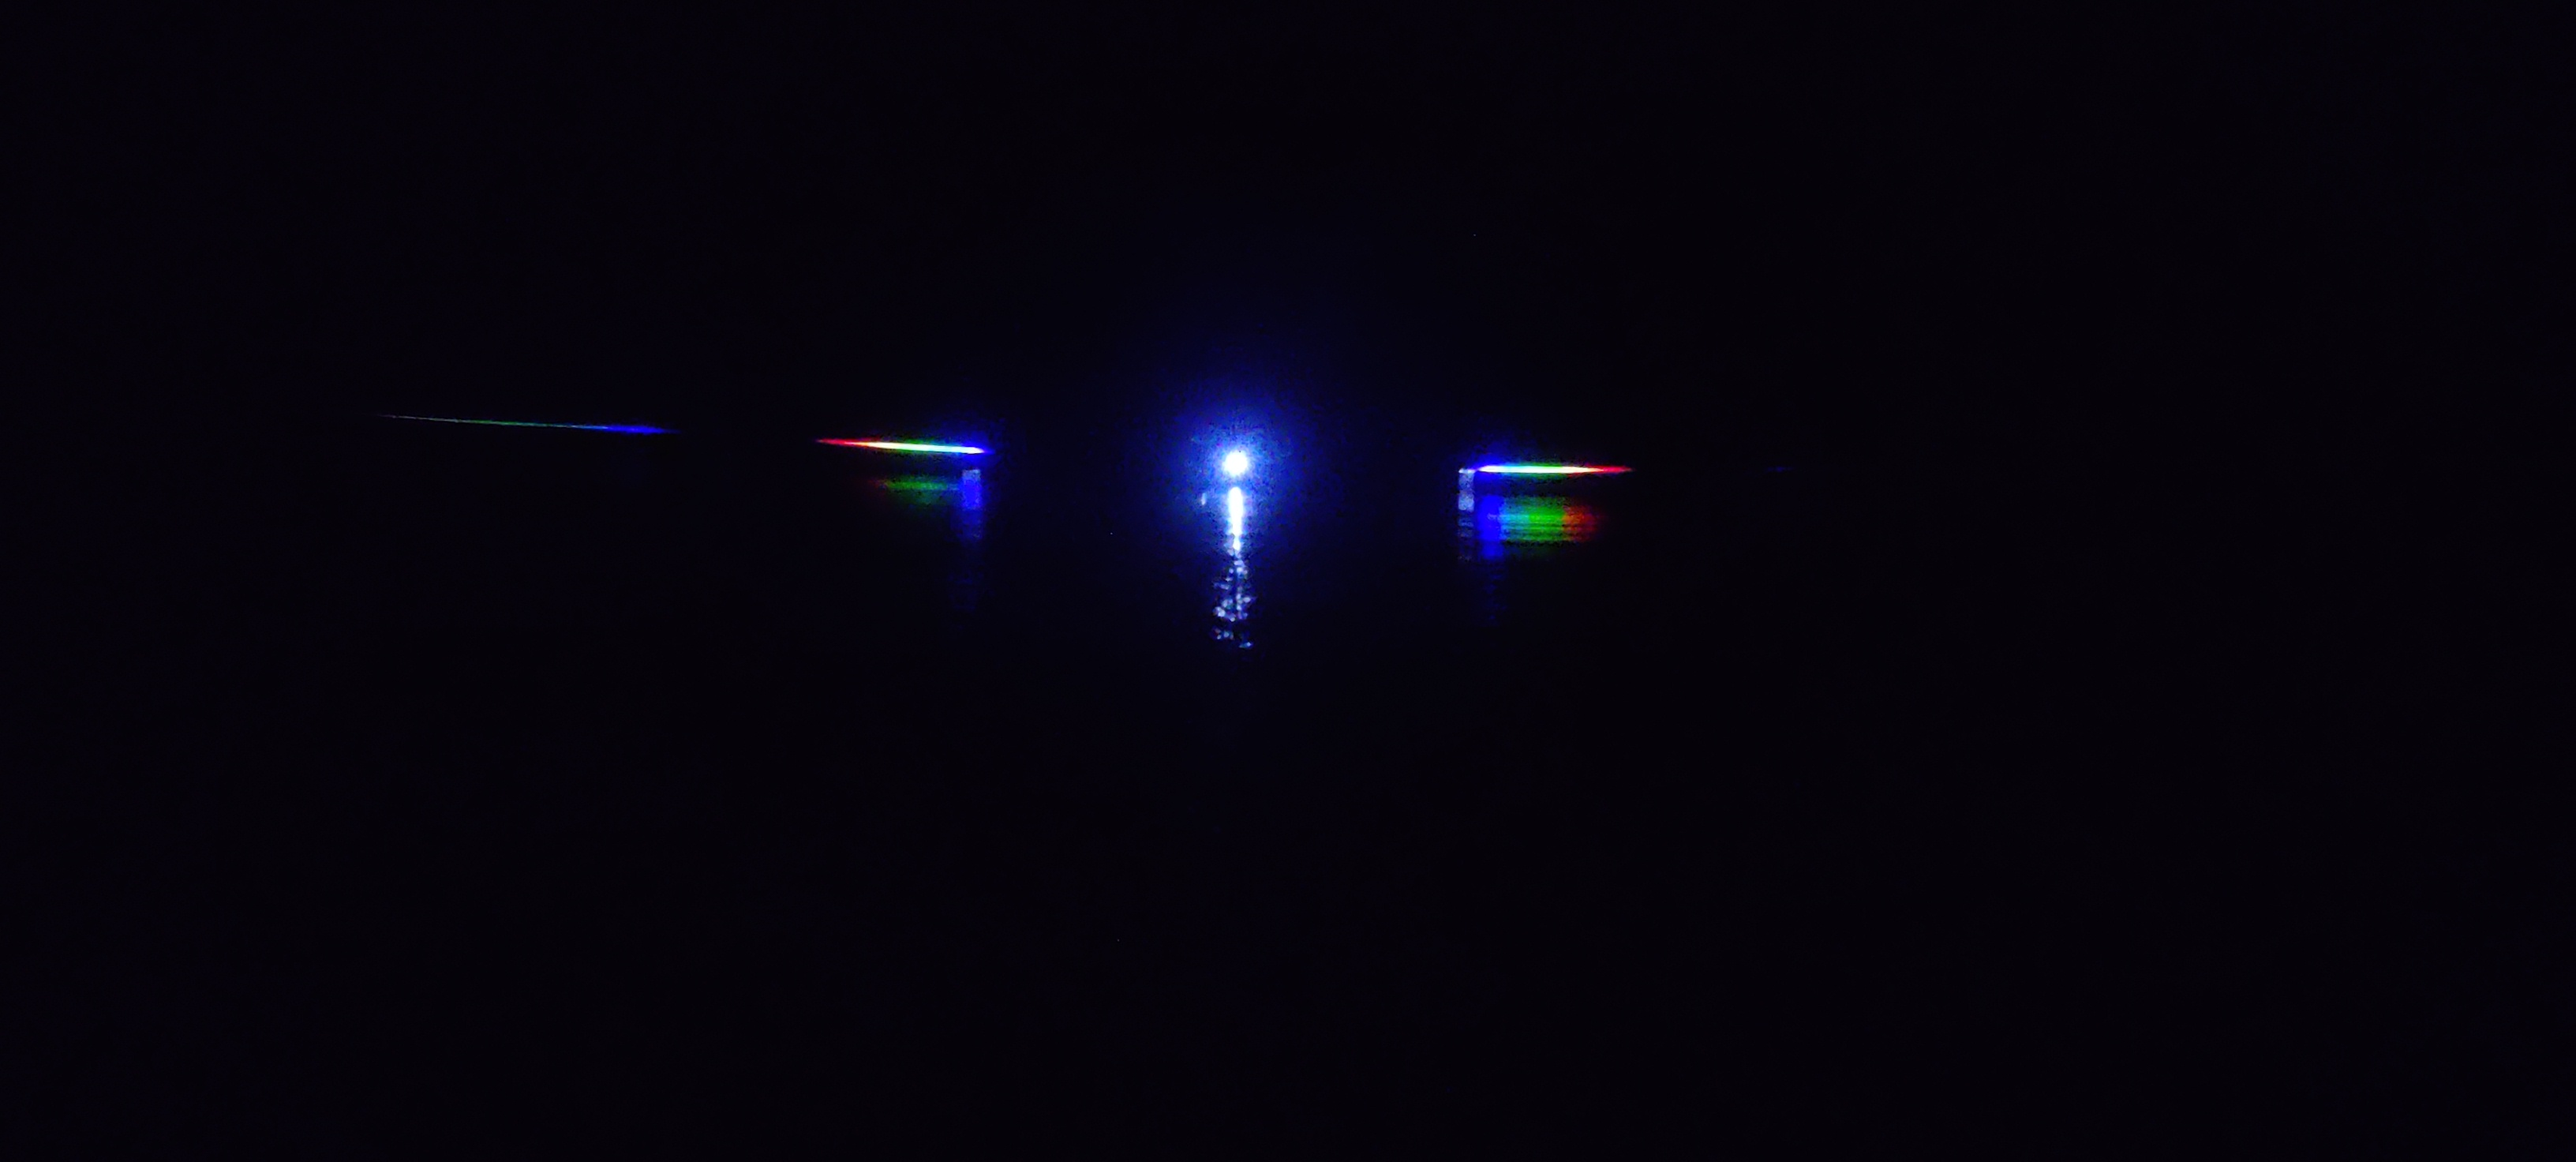
\includegraphics[width=0.7\linewidth]{LedCorto1_OFF.jpg}
    \caption{Foto diffrazione puntatore su reticolo corto}
    \label{LedCorto}
\end{figure}

\clearpage

Effettuate queste misure è stata scattata una foto a luce spenta della diffrazione del puntatore sul reticolo corto (Figura \ref{LedCorto}), avente una densità di fenditure per millimetro pari a $\rho_{corto} = 500 \pm 1\; fend/mm $ e quindi un passo di $d_{corto} = 2,000 \pm 0,004 \; \mu m $. Erano visibili  gli spettri del primo ordine da ambo i lati e del secondo ordine solo a destra, che si è deciso di non analizzare.

\vspace{3mm}

Si è proceduto a misurare i $ \Delta x $ con \textit{ImageJ} ottenendo quanto riportato in Tabella 3 e 4.

\begin{table}[h]
        \centering
        \begin{tabular}{||c|c|c|c|c|c||}
            \hline
            \# & \cellcolor{blue}$\Delta x_{blu}$ [m] & \cellcolor{cyan}$\Delta x_{ciano}[m]$ & \cellcolor{green}$\Delta x_{verde}[m]$ & \cellcolor{orange}$\Delta x_{arancio}[m]$ & \cellcolor{red}$\Delta x_{rosso}[m]$ \\
            \hline
            1 & 0,998 & 1,098 & 1,208 & 1,325 & 1,485 \\
            2 & 0,998 & 1,094 & 1,210 & 1,362 & 1,510 \\
            3 & 0,994 & 1,078 & 1,210 & 1,352 & 1,494 \\
            \hline
        \end{tabular}
        \caption{Misura del primo ordine a sinistra}
    \centering
    \begin{tabular}{||c|c|c|c|c|c||}
        \hline
        \# & \cellcolor{blue}$\Delta x_{blu}$ [m] & \cellcolor{cyan}$\Delta x_{ciano}[m]$ & \cellcolor{green}$\Delta x_{verde}[m]$ & \cellcolor{orange}$\Delta x_{arancio}[m]$ & \cellcolor{red}$\Delta x_{rosso}[m]$ \\
        \hline
        1 & 0,996 & 1,038 & 1,162 & 1,288 & 1,398 \\
        2 & 0,965 & 1,051 & 1,164 & 1,304 & 1,407\\
        3 & 0,963 & 1,054 & 1,156 & 1,282 & 1,400 \\
        \hline
    \end{tabular}
    \caption{Misura del primo ordine a destra}
\end{table}


Siccome l'analisi dati viene fatta con un programma controllato dall'utente e non da un algoritmo, mi è sembrato inopportuno limitarmi a propagare l'errore di $L$ e $z$. Infatti ci possono essere state molteplici sorgenti di errore. Il reticolo poteva non essere perfettamente ortogonale con fotocamera e sorgente, o non alla stessa altezza da terra nonostante la massima attenzione posta. Questo si nota nel fatto che le misure di sinistra siano leggermente più grandi di quelle a destra (proprio per questa ragione non è stato analizzato lo spettro del secondo ordine di sinistra; non era presente uno spettro di destra che potesse compensare lo spostamento verso l'alto dei $\Delta x$ di cui verrà successivamente fatta una media). 

\vspace{3mm}

Una causa alternativa di questo errore sistematico può essere stata una angolazione della fotocamera rispetto al reticolo, dovuta al tocco per scattare. Inoltre i $\Delta x$ sono stati misurati con \textit{ImageJ} a gruppi di 5, uno per colore, tenendo fisso un estremo di misura sulla sorgente e muovendo l'altro, per poi riposizionare anche l'estremo della sorgente e ripetere il procedimento. Questa scelta è stata adottata per evitare errori dovuti a un errato posizionamento dell'estremo sulla sorgente. Ciononostante la sorgente e gli spettri risultano molto espansi, anche a causa dei riflessi contro le superfici lucide, e quindi un errore può comunque derivare da questo.

\vspace{3mm}

In generale queste problematiche, che in gran parte nascono dagli strumenti rudimentali a disposizione per organizzare l'ambiente e le misure, mi hanno fatto ritenere che la scelta più adatta fosse definire l'incertezza dei $\Delta x$ come deviazione standard delle 6 misure totali prese per ogni colore. L'incertezza così facendo aumenta e riesce a tenere maggiormente conto di tutte le possibili fonti di errore.

\vspace{3mm}

La scelta di usare la deviazione standard per le misure di $\Delta x$ è una costante in questo esperimento.

\vspace{3mm}

I risultati ottenuti per i $\Delta x$  medi $\overline{\Delta x}$ sono riportati in Tabella 5.

\begin{table}[h]
    \centering
\begin{tabular}{||c|c|c|c|c|c||}
    \hline
     & \cellcolor{blue}$\overline{\Delta x_{blu}}$ [m] & \cellcolor{cyan}$\overline{\Delta x_{ciano}} [m]$ & \cellcolor{green}$\overline{\Delta x_{verde}}[m]$ & \cellcolor{orange}$\overline{\Delta x_{arancio}}[m]$ & \cellcolor{red}$\overline{\Delta x_{rosso}}[m]$ \\
    \hline
    Media & 0,981 & 1,069 & 1,185 & 1,319 & 1,449 \\
    $\sigma$ & 0,016 & 0,023 & 0,024 & 0,030 & 0,048\\
    \hline
\end{tabular}
\caption{$\Delta x$ medi per diffrazione del puntatore sul reticolo corto}
\end{table}

\pagebreak 
Da qui usando l'Equazione (\ref{first_order_equation}) se ne sono ricavate le $\lambda$ riportate in Tabella 6.

\begin{table}[h]
    \centering
\begin{tabular}{||c|c|c|c|c|c||}
    \hline
     & \cellcolor{blue}$\lambda_{blu}$ [nm] & \cellcolor{cyan}$\lambda_{ciano} [nm]$ & \cellcolor{green}$\lambda_{verde}[nm]$ & \cellcolor{orange}$\lambda_{arancio}[nm]$ & \cellcolor{red}$\lambda_{rosso}[nm]$ \\
    \hline
    Media & 442,6 & 482,4 & 534,8 & 595,2 & 654,0 \\
    $\sigma$ & 7,4 & 10,3 & 11,2 & 13,8 & 21,7\\
    \hline
\end{tabular}
\caption{$\lambda$ per diffrazione del puntatore sul reticolo corto}
\end{table}

L'errore su $\lambda$ è stato ricavato con la propagazione degli errori:

\begin{equation}
        \sigma_\lambda =  \sqrt{\left(\frac{\Delta x}{z}\cdot\sigma_z\right)^2 + \left(\frac{d}{z}\cdot\sigma_{\Delta x}\right)^2 + \left(\frac{z \lambda}{\Delta x^2}\cdot\sigma_{\Delta x}\right)^2}
    \label{lambda_error}
\end{equation}

\vspace{3mm}

Si precisa che i LED (Light Emitting Diode) per illuminazione seguono la tecnologia RGB, ovvero emettono luce apparentemente bianca con il solo ausilio dei colori rosso, verde e blu. Pertanto è altamente probabile che il ciano e l'arancione siano dei colori posizionati correttamente nello spettro, ma percepiti in quanto la diffrazione è solo al primo ordine. Per ordini superiori questi colori dovrebbero scomparire o perdere molta intensità.


%%% -----------------------------------------------------------------------------------------------------%

\subsection{Calcolo \textrm{$d_{lungo}$}}

Mantendo invariata la sorgente si è rimosso il reticolo corto in favore di quello lungo, di passo ignoto. Si è misurata per 7 volte la distanza $z$ tra reticolo e sorgente, ottenendo i dati riportati in Tabella 7.

\begin{table}[h]
    \centering
        \begin{tabular}{||c|c|c||}
            \hline
            \# & $z [m]$ & $\sigma_z [m]$\\
            \hline
            1 & 4,44 & 0,01 \\
            2 & 4,44 & 0,01 \\
            3 & 4,43 & 0,01 \\
            4 & 4,43 & 0,01 \\
            5 & 4,45 & 0,01 \\
            6 & 4,45 & 0,01 \\
            7 & 4,43 & 0,01 \\
            \hline
            $z_{best}$ & 4,44 & 0,01 \\
            \hline
        \end{tabular}
    \caption{Misura di $z$}
\end{table}

La fotocamera è stata riposizionata dietro al reticolo e si è verificata l'ortogonalità sorgente - reticolo - fotocamera per quanto possibile. Per questa misura sono state scattate due coppie di foto luce-buio, e pertanto sono state analizzate un totale di 2 immagini di diffrazione, ottenendo 12 valori per colore di $\Delta x$. L'analisi ha seguito i criteri spiegati nella sezione precedente. Era visibile solo lo spettro del primo ordine da ambo i lati.

\begin{figure}[h]
    \centering
    \begin{subfigure}[b]{0.4\linewidth}
        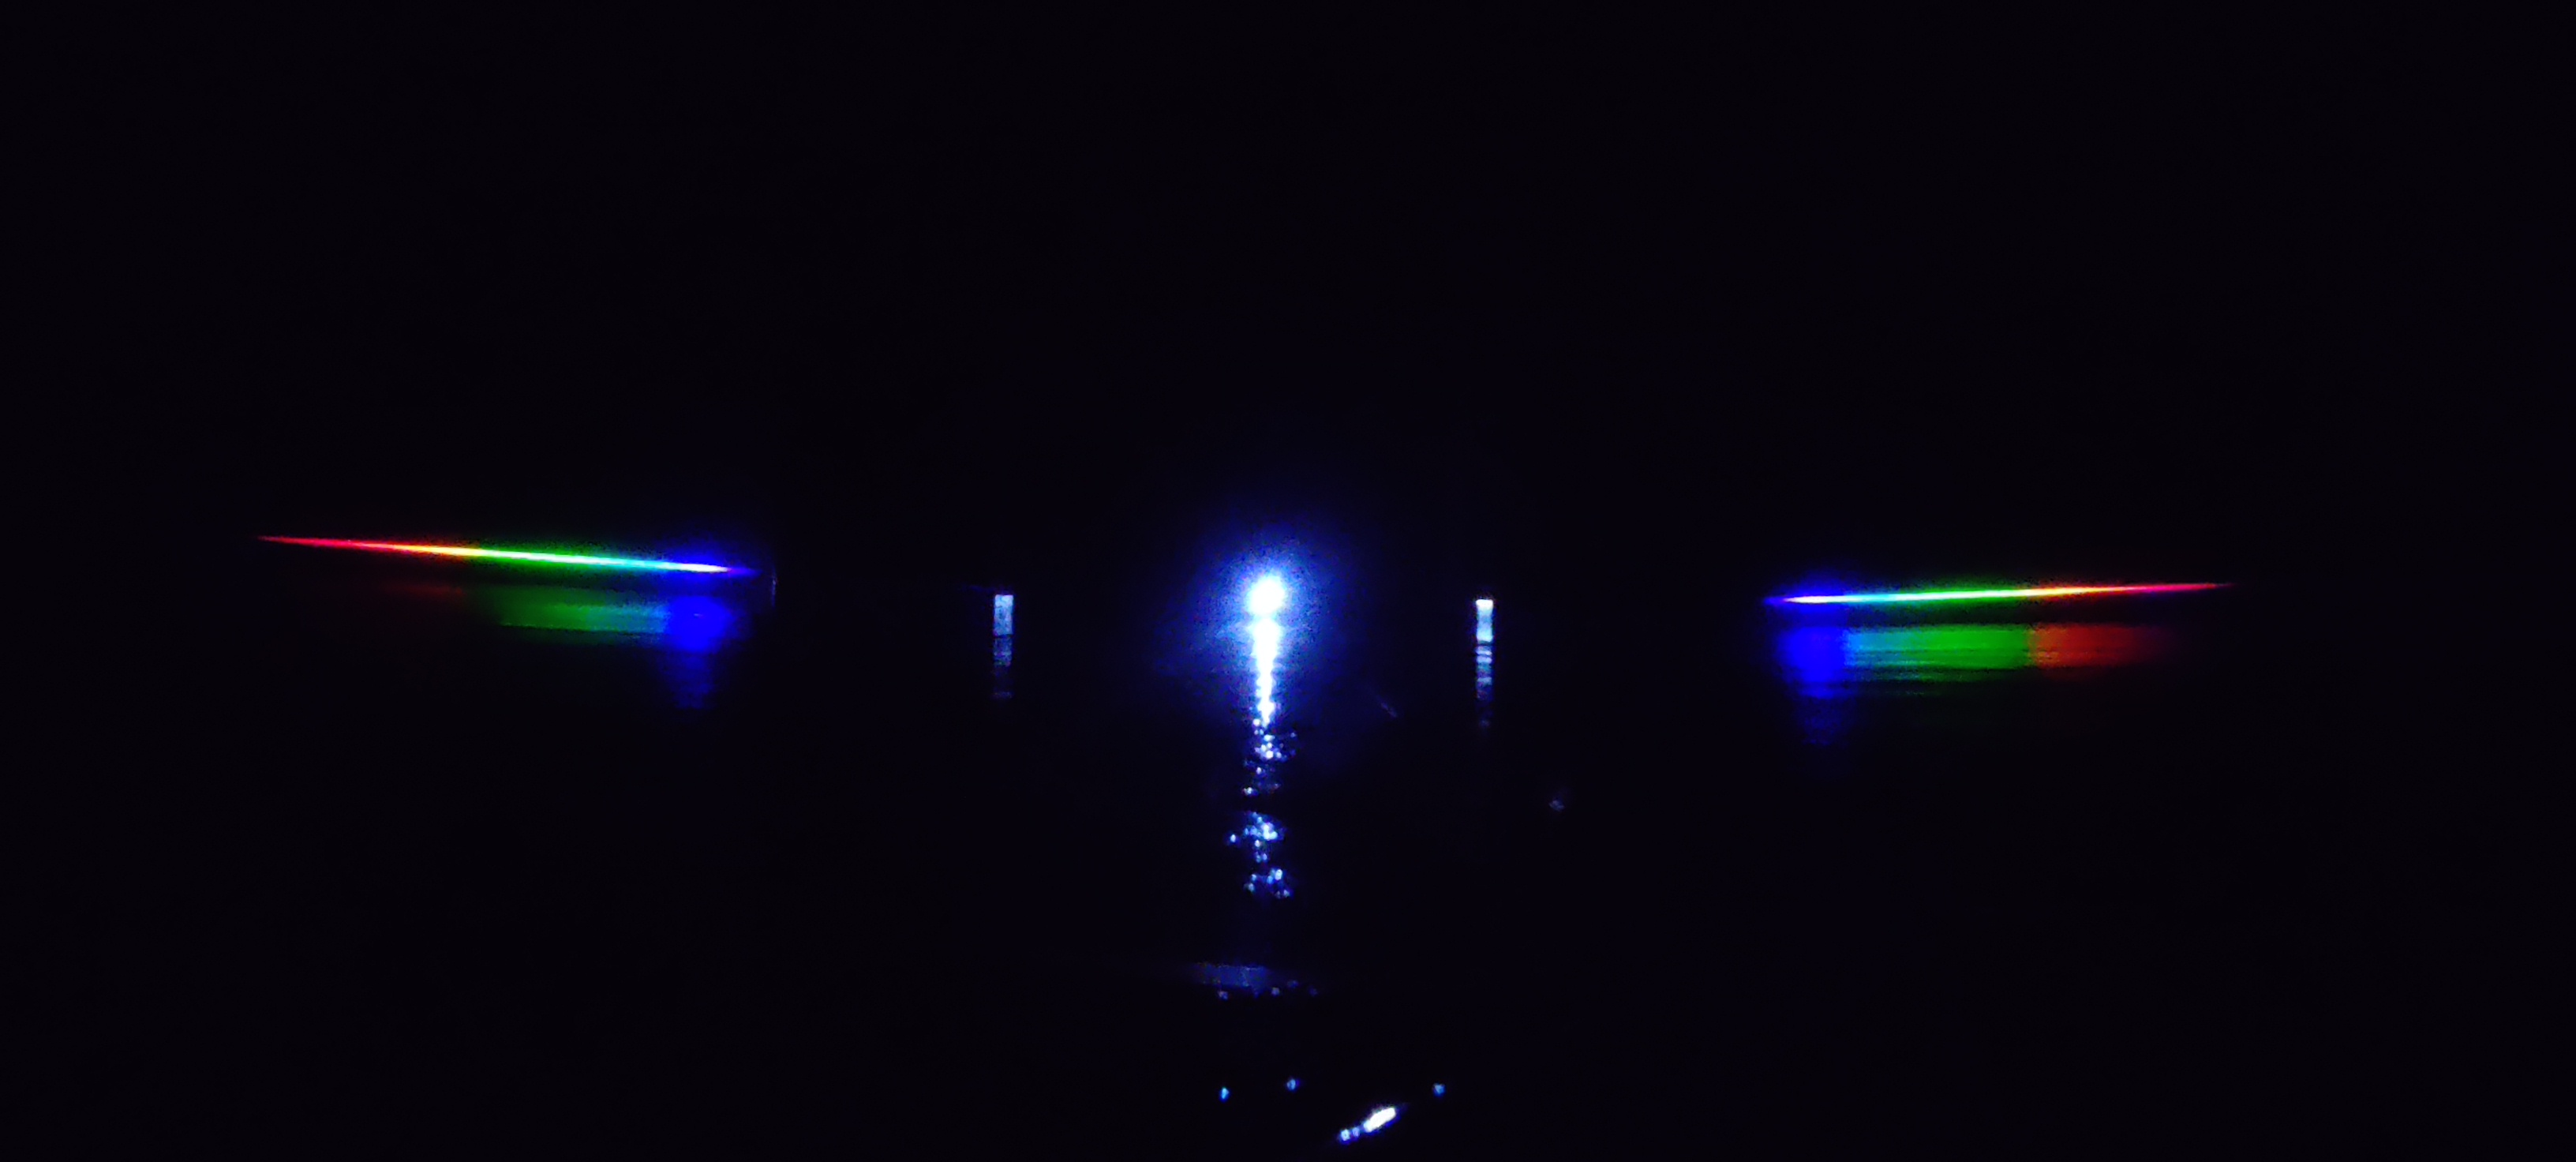
\includegraphics[width=\linewidth]{LedLungo1_OFF.jpg}
        \caption{Scatto 1}
    \end{subfigure}

    \begin{subfigure}[b]{0.4\linewidth}
        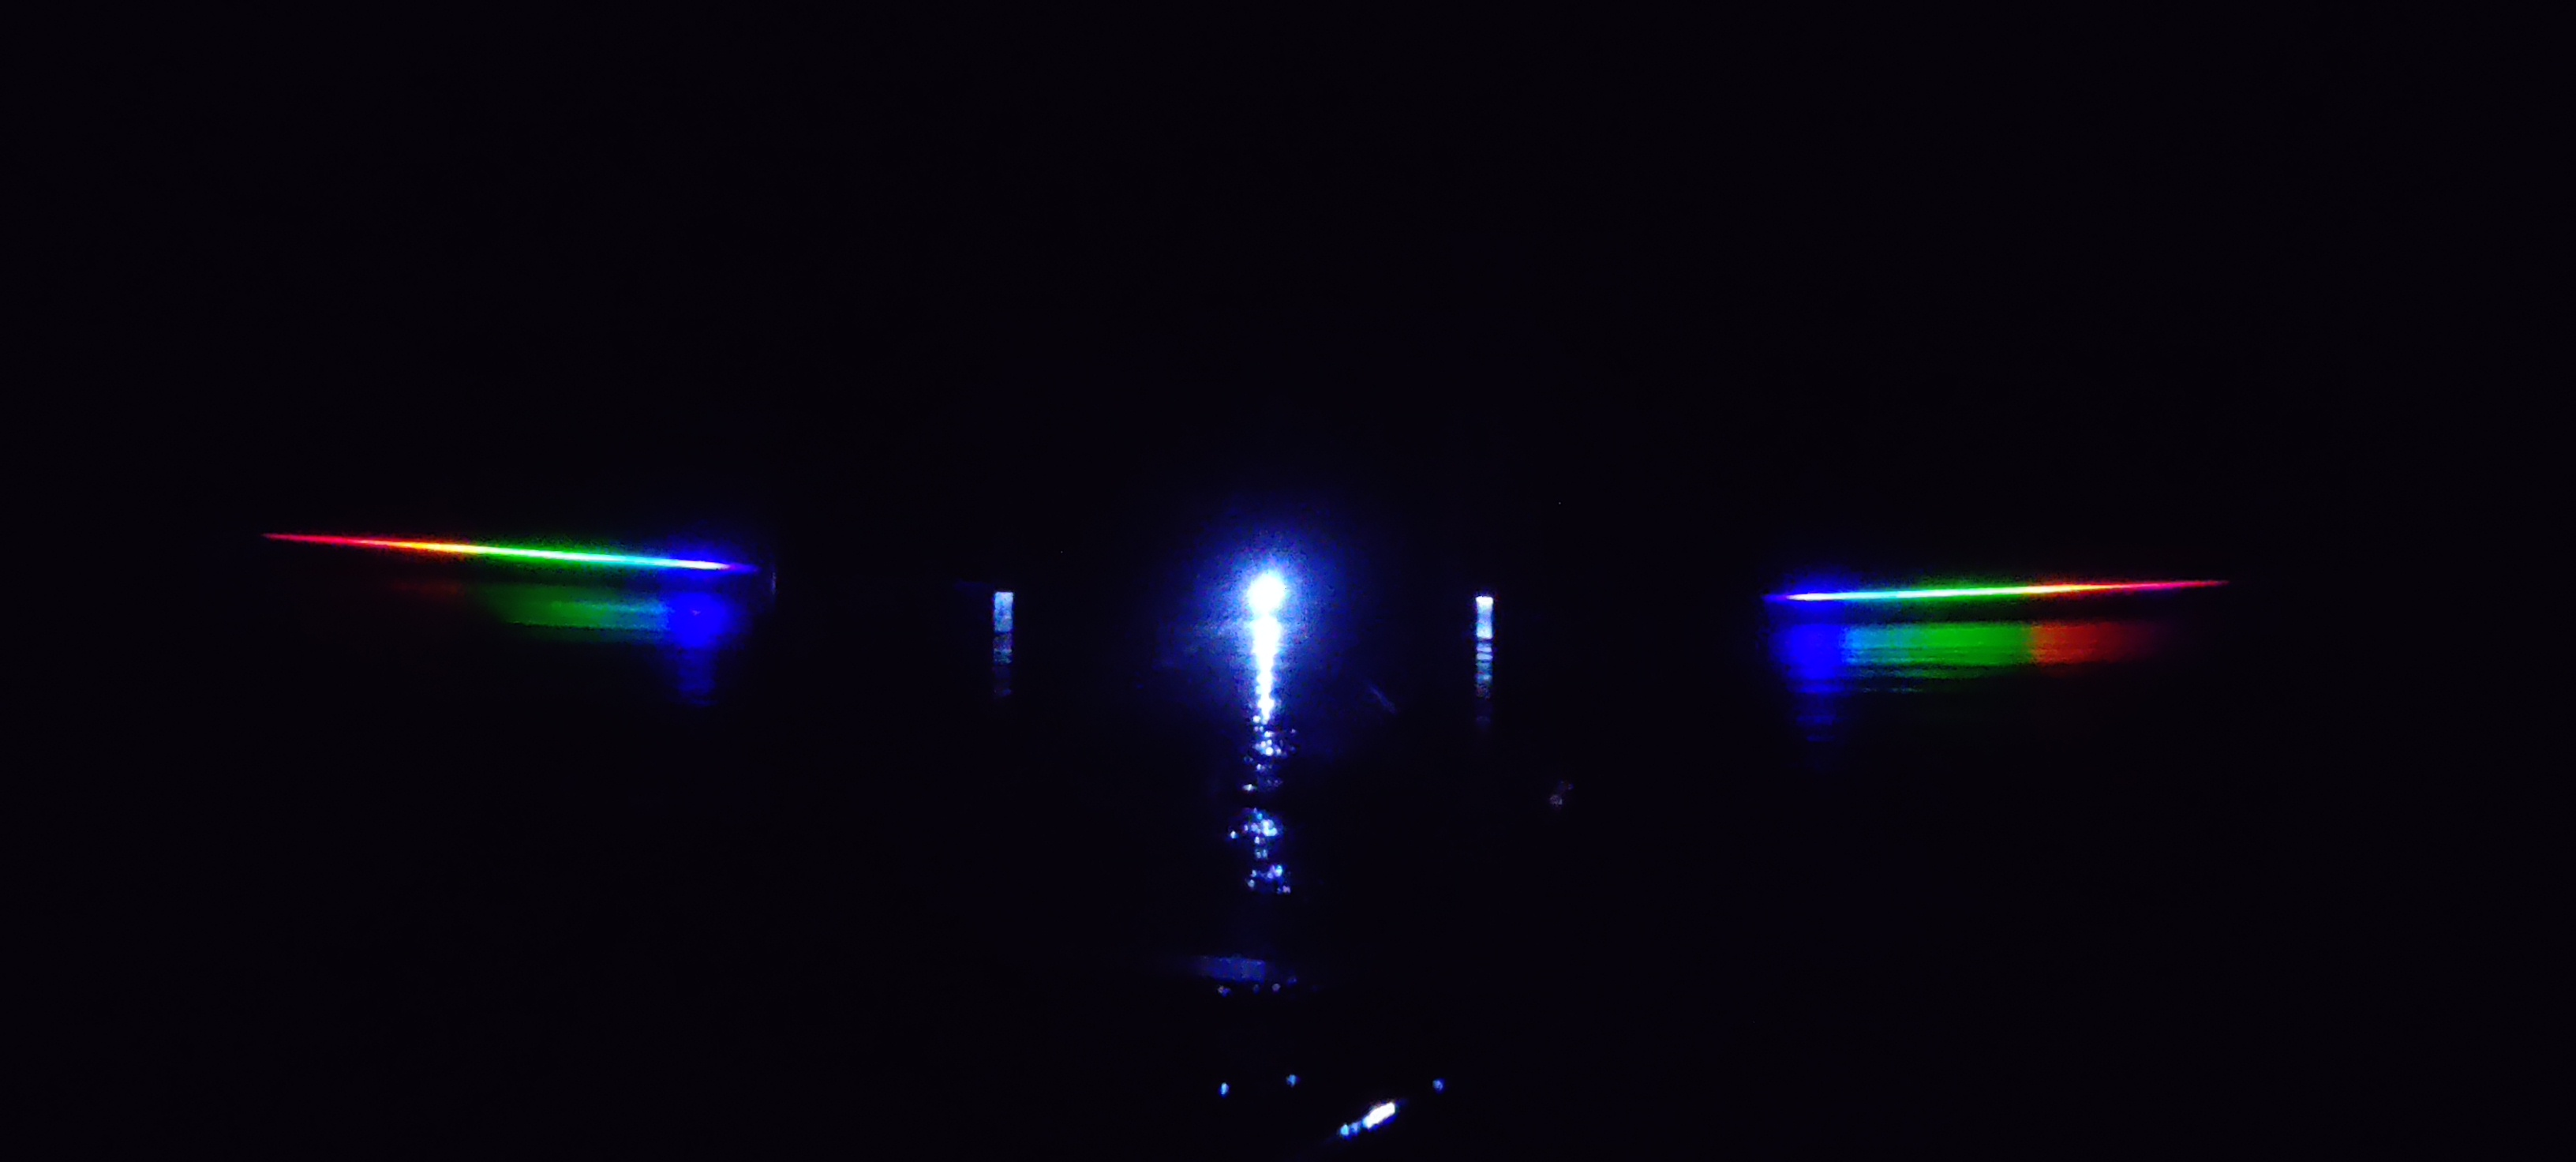
\includegraphics[width=\linewidth]{LedLungo3_OFF.jpg}
        \caption{Scatto 2}
    \end{subfigure}
    \caption{Due scatti della diffrazione tra puntatore e reticolo lungo, solo in apparenza perfettamente identici}
\end{figure}
\pagebreak
I valori ottenuti per $\Delta x$ sono riportati in Tabelle 8 e 9

\begin{table}[h]
    \centering
    \begin{tabular}{||c|c|c|c|c|c|c||}
        \hline
        Foto & \# & \cellcolor{blue}$\Delta x_{blu}$ [m] & \cellcolor{cyan}$\Delta x_{ciano}[m]$ & \cellcolor{green}$\Delta x_{verde}[m]$ & \cellcolor{orange}$\Delta x_{arancio}[m]$ & \cellcolor{red}$\Delta x_{rosso}[m]$ \\
        \hline
        Scatto 1 & 1 & 2,300 & 2,600 & 2,959 & 3,409 & 3,749 \\
        Scatto 1 & 2 & 2,309 & 2,575 & 2,932 & 3,406 & 3,766 \\
        Scatto 1 & 3 & 2,274 & 2,572 & 2,935 & 3,401 & 3,827 \\
        Scatto 2 & 4 & 2,241 & 2,486 & 2,853 & 3,333 & 3,741 \\
        Scatto 2 & 5 & 2,233 & 2,494 & 2,830 & 3,310 & 3,743 \\
        Scatto 2 & 6 & 2,239 & 2,475 & 2,870 & 3,303 & 3,737 \\
        \hline
    \end{tabular}
    \caption{Misura del primo ordine a sinistra}
\centering
\begin{tabular}{||c|c|c|c|c|c|c||}
    \hline
    Foto & \# & \cellcolor{blue}$\Delta x_{blu}$ [m] & \cellcolor{cyan}$\Delta x_{ciano}[m]$ & \cellcolor{green}$\Delta x_{verde}[m]$ & \cellcolor{orange}$\Delta x_{arancio}[m]$ & \cellcolor{red}$\Delta x_{rosso}[m]$ \\
    \hline
    Scatto 1 & 1 & 2,232 & 2,450 & 2,821 & 3,299 & 3,638 \\
    Scatto 1 & 2 & 2,235 & 2,479 & 2,799 & 3,273 & 3,683 \\
    Scatto 1 & 3 & 2,232 & 2,479 & 2,809 & 3,292 & 3,686 \\
    Scatto 2 & 4 & 2,177 & 2,399 & 2,778 & 3,207 & 3,577 \\
    Scatto 2 & 5 & 2,170 & 2,430 & 2,775 & 3,191 & 3,614 \\
    Scatto 2 & 6 & 2,173 & 2,377 & 2,765 & 3,188 & 3,611 \\
    \hline
\end{tabular}
\caption{Misura del primo ordine a destra}
\end{table}

\clearpage
Da cui si sono ottenuti dei valori medi $\overline{\Delta x}$ riportati in Tabella 10.

\begin{table}[h]
    \centering
\begin{tabular}{||c|c|c|c|c|c||}
    \hline
     & \cellcolor{blue}$\overline{\Delta x_{blu}}$ [m] & \cellcolor{cyan}$\overline{\Delta x_{ciano}} [m]$ & \cellcolor{green}$\overline{\Delta x_{verde}}[m]$ & \cellcolor{orange}$\overline{\Delta x_{arancio}}[m]$ & \cellcolor{red}$\overline{\Delta x_{rosso}}[m]$ \\
    \hline
    Media & 2,235 & 2,485 & 2,844 & 3,301 & 3,698 \\
    $\sigma$ & 0,044 & 0,066 & 0,064 & 0,075 & 0,072\\
    \hline
\end{tabular}
\caption{$\Delta x$ medi per diffrazione del puntatore sul reticolo lungo}
\end{table}

É curioso notare come anche in questo caso i $\Delta x$ misurati a destra abbiano valori leggermente maggiori di quelli misurati a sinistra, a riprova del fatto che è molto difficile raggiungere una perfetta ortogonazzazione tra le varie parti dell'apparato senza l'ausilio di strumenti professionali.

\vspace{3mm}

Avendo già ricavato le lunghezze d'onda emesse dal puntatore, come riportato in Tabella 6, è possibile utilizzare nuovamente l'Equazione (\ref{first_order_equation}) per ricavare il passo $d$ del reticolo lungo da ogni $\lambda$. Sono riportati in Tabella 11 i curiosi risultati, la cui incertezza è ricavata mediante la propagazione degli errori:

\begin{equation}
    \sigma_d = \sqrt{\left(\frac{\lambda}{\Delta x}\cdot\sigma_z\right)^2 + \left(\frac{z}{\Delta x}\cdot\sigma_\lambda\right)^2 + \left(\frac{z \lambda}{\Delta x^2}\cdot\sigma_{\Delta x}\right)^2}
\end{equation}

\begin{table}[h]
    \centering
\begin{tabular}{||c|c|c|c|c|c||}
    \hline
     & \cellcolor{blue}$d_{blu}$ [nm] & \cellcolor{cyan}$d_{ciano} [nm]$ & \cellcolor{green}$d_{verde}[nm]$ & \cellcolor{orange}$d_{arancio}[nm]$ & \cellcolor{red}$d_{rosso}[nm]$ \\
    \hline
    Media & 0,879 & 0,861 & 0,835 & 0,800 & 0,785 \\
    $\sigma$ & 0,023 & 0,029 & 0,026 & 0,026 & 0,030\\
    \hline
\end{tabular}
\caption{Passo del reticolo lungo}
\end{table}

Definisco curiosi i risultati poichè rappresentano approssimativamente una retta con pendenza negativa (Figura \ref{graph_d}). Considerando che $z$ nell'Equazione (\ref{first_order_equation}) è uguale per ogni passo calcolato, il problema di queste misure è necessariamente generato o dalle $\lambda$ misurate con il reticolo corto o dai $\Delta x$ del reticolo lungo. Ritengo che l'errore sia da imputare all'analisi delle foto con il software. 

\vspace{3mm}

Infatti, prendendo come esempio la Figura \ref{LedCorto}, il blu risulta molto corto in termini di lunghezza nello spettro ma anche molto luminoso, rendendo difficile ad esempio misurarne sempre il punto medio. Invece il verde è molto lungo e il suo punto medio è quindi più facile da misurare, mentre l'arancio quasi si mescola con il rosso e non presenta un confine abbastanza definito.

\vspace{3mm}

Al netto di queste considerazioni su quale possa essere la causa dell'errore e che, essendo proprio l'analisi dell'immagine, inevitabilmente colpisce sia le $\lambda$ che i $\Delta x$, ho deciso di procedere con una media aritmetica con incertezza la deviazione standard per avere una stima del passo del reticolo.

\begin{figure}[h]
    \centering
    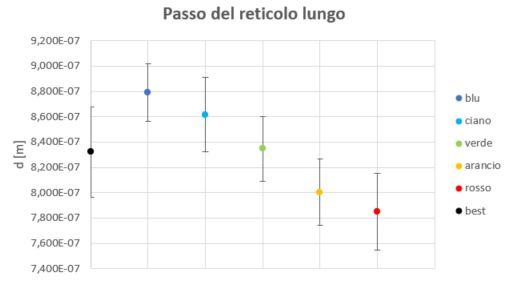
\includegraphics[width=0.6\linewidth]{graph_d.JPG}
    \caption{Grafico dei valori del passo del reticolo lungo ottenuti dalle varie lunghezze d'onda}
    \label{graph_d}
\end{figure}

\vspace{3mm}

Il valore ottenuto è 

\[d_{lungo} = 0,832 \pm 0,036 \; nm\]

che corrisponde a una densità di fenditure per millimetro $\rho = 0,001/(d_{lungo}\cdot 10^{-6}) \; fend/mm $

\[\rho_{lungo} = 1202 \pm 51 \; fend/mm\]

con un errore di circa il 4\%, che considero quantomeno accettabile per i pochi mezzi a disposizione.

%%% LUNGHEZZE D'ONDA EMESSE DA TORCIA A LED %%%
\section{Calcolo lunghezze d'onda emesse dalla torcia}
Dopo avere determinato il passo del reticolo lungo, ho misurato le lunghezze d'onda emesse da una torcia a led con entrambi i reticoli, per poterne confrontare i risultati.

\subsection{Reticolo corto}
Dopo avere riposizionato il reticolo corto a una distanza $z = 4,43 \pm 0,01 \; m$ (come riportato in Tabella 12), avere posizionato la torcia sulla destra del vocabolario e con il punto di emissione della luce complanare al vocabolario, essermi nuovamente assicurato che i componenti del sistema fossero ortogonali tra loro ed equidistanti dal suolo, ho iniziato la misura.

\begin{table}[h]
    \centering
        \begin{tabular}{||c|c|c||}
            \hline
            \# & $z [m]$ & $\sigma_z [m]$\\
            \hline
            1 & 4,43 & 0,01 \\
            2 & 4,42 & 0,01 \\
            3 & 4,43 & 0,01 \\
            4 & 4,44 & 0,01 \\
            5 & 4,45 & 0,01 \\
            6 & 4,42 & 0,01 \\
            7 & 4,43 & 0,01 \\
            \hline
            $z_{best}$ & 4,43 & 0,01 \\
            \hline
        \end{tabular}
    \caption{Misura di $z$}
\end{table}


\vspace{3mm}

Ho proceduto come già spiegato nelle sezioni precedenti, raccogliendo una sola coppia di foto luce-buio, ma in cui erano ben visibili gli spettri del secondo ordine da ambo i lati. Questo mi permette, a differenza di come fatto in Sezione \ref{3.1}, di potere misurare i $\Delta x$ anche al secondo ordine.
\pagebreak
\begin{figure}[h]
    \centering
    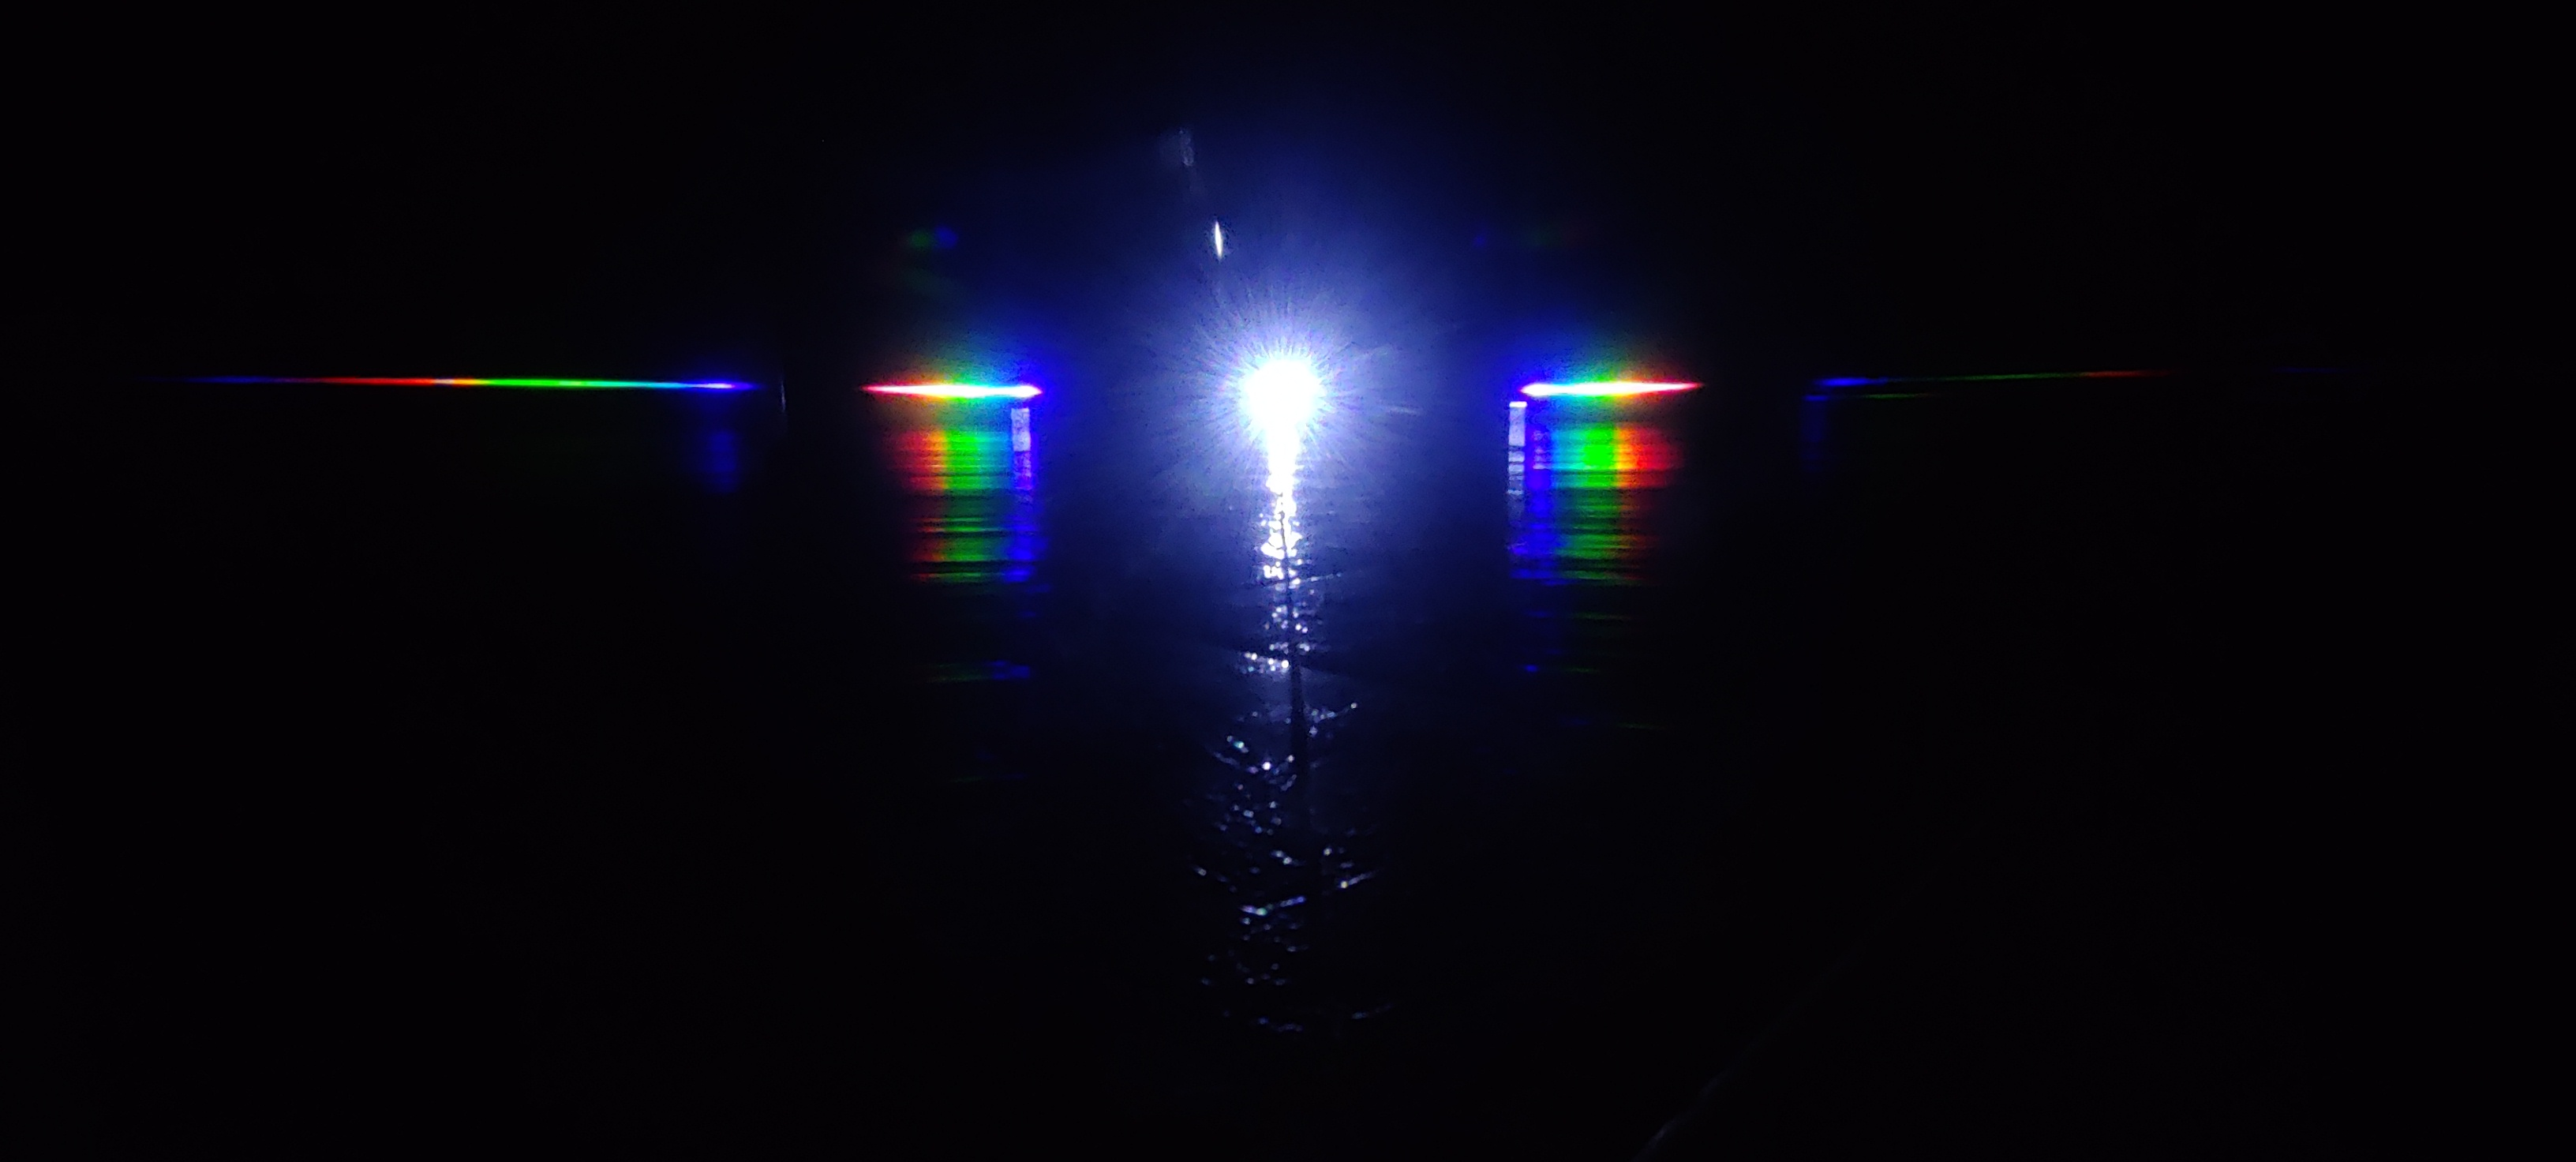
\includegraphics[width=0.7\linewidth]{TorciaCorto5_OFF.jpg}
    \caption{Diffrazione della torcia su reticolo corto. Ben visibili gli spettri del secondo ordine}
    \label{TorciaCorto}
\end{figure}

Osservando la Figura \ref{TorciaCorto} si nota subito un dettaglio molto interessante. 

\vspace{3mm}

Il secondo ordine a destra è poco luminoso e presenta solo i colori tipici del sistema RGB, il che conferma il fatto che le altre tonalità siano solo un mescolamento di rosso, verde e blu. 
Il secondo ordine a sinistra invece è molto più luminoso e presenta molti più colori. 

\vspace{3mm}

Una spiegazione plausibile è che la presenza di una vetrina sul lato sinistro della stanza (esattamente dove cade questo spettro) abbia enormemente favorito riflessioni dal pavimento lucido e dalla sorgente stessa, generando uno spettro molto simile al primo ordine per quantità di colori presenti e intensità.

\vspace{3mm}

L'analisi software degli spettri del primo ordine ha prodotto i valori $\Delta x$ riportati nelle Tabelle 13 e 14

\begin{table}[h]
    \centering
    \begin{tabular}{||c|c|c|c|c|c||}
        \hline
        \# & \cellcolor{blue}$\Delta x_{blu}$ [m] & \cellcolor{cyan}$\Delta x_{ciano}[m]$ & \cellcolor{green}$\Delta x_{verde}[m]$ & \cellcolor{orange}$\Delta x_{arancio}[m]$ & \cellcolor{red}$\Delta x_{rosso}[m]$ \\
        \hline
        1 & 1,012 & 1,106 & 1,244 & 1,375 & 1,538 \\
        2 & 1,012 & 1,125 & 1,261 & 1,399 & 1,542 \\
        3 & 1,018 & 1,122 & 1,258 & 1,403 & 1,550 \\
        \hline
    \end{tabular}
    \caption{Misura del primo ordine a sinistra}
\centering
\begin{tabular}{||c|c|c|c|c|c||}
    \hline
    \# & \cellcolor{blue}$\Delta x_{blu}$ [m] & \cellcolor{cyan}$\Delta x_{ciano}[m]$ & \cellcolor{green}$\Delta x_{verde}[m]$ & \cellcolor{orange}$\Delta x_{arancio}[m]$ & \cellcolor{red}$\Delta x_{rosso}[m]$ \\
    \hline
    1 & 1,000 & 1,107 & 1,227 & 1,355 & 1,495 \\
    2 & 1,001 & 1,097 & 1,219 & 1,342 & 1,502\\
    3 & 0,993 & 1,086 & 1,210 & 1,326 & 1,499 \\
    \hline
\end{tabular}
\caption{Misura del primo ordine a destra}
\end{table}

Aventi valori medi $\overline{\Delta x}$ riportati in Tabella 15.

\begin{table}[h]
    \centering
\begin{tabular}{||c|c|c|c|c|c||}
    \hline
     & \cellcolor{blue}$\overline{\Delta x_{blu}}$ [m] & \cellcolor{cyan}$\overline{\Delta x_{ciano}} [m]$ & \cellcolor{green}$\overline{\Delta x_{verde}}[m]$ & \cellcolor{orange}$\overline{\Delta x_{arancio}}[m]$ & \cellcolor{red}$\overline{\Delta x_{rosso}}[m]$ \\
    \hline
    Media & 1,006 & 1,107 & 1,237 & 1,367 & 1,521 \\
    $\sigma$ & 0,009 & 0,013 & 0,019 & 0,028 & 0,023 \\
    \hline
\end{tabular}
\caption{$\Delta x$ medi per diffrazione della torcia sul reticolo corto, ricavate dagli spettri del primo ordine}
\end{table}
\pagebreak
Da cui sono state ricavate le lunghezze d'onda riportate in Tabella 16.

\begin{table}[h]
    \centering
\begin{tabular}{||c|c|c|c|c|c||}
    \hline
     $m = 1$ & \cellcolor{blue}$\lambda_{blu}$ [nm] & \cellcolor{cyan}$\lambda_{ciano} [nm]$ & \cellcolor{green}$\lambda_{verde}[nm]$ & \cellcolor{orange}$\lambda_{arancio}[nm]$ & \cellcolor{red}$\lambda_{rosso}[nm]$ \\
    \hline
    Media & 454,0 & 499,7 & 558,1 & 616,8 & 686,5 \\
    $\sigma$ & 4,1 & 6,3 & 8,8 & 12,9 & 10,5\\
    \hline
\end{tabular}
\caption{$\lambda$ per diffrazione della torcia sul reticolo corto, calcolate dagli spettri al primo ordine}
\end{table}


Al secondo ordine invece sono state raccolte e analizzate le misure riportate in Tabelle 17, 18, 19, 20.

\begin{table}[h]
    \centering
    \begin{tabular}{||c|c|c|c|c|c||}
        \hline
        \# & \cellcolor{blue}$\Delta x_{blu}$ [m] & \cellcolor{cyan}$\Delta x_{ciano}[m]$ & \cellcolor{green}$\Delta x_{verde}[m]$ & \cellcolor{orange}$\Delta x_{arancio}[m]$ & \cellcolor{red}$\Delta x_{rosso}[m]$ \\
        \hline
        1 & 2,216 & 2,451 & 2,936 & 3,243 & 3,553 \\
        2 & 2,225 & 2,439 & 2,877 & 3,268 & 3,544 \\
        3 & 2,228 & 2,492 & 2,942 & 3,277 & 3,559 \\
        \hline
    \end{tabular}
    \caption{Misura del secondo ordine a sinistra}
\centering
\begin{tabular}{||c|c|c|c|c|c||}
    \hline
    \# & \cellcolor{blue}$\Delta x_{blu}$ [m] & \cellcolor{cyan}$\Delta x_{ciano}[m]$ & \cellcolor{green}$\Delta x_{verde}[m]$ & \cellcolor{orange}$\Delta x_{arancio}[m]$ & \cellcolor{red}$\Delta x_{rosso}[m]$ \\
    \hline
    1 & 2,226 & & 2,840 & & 3,321 \\
    2 & 2,241 & & 2,803 & & 3,340 \\
    3 & 2,235 & & 2,818 & & 3,334 \\
    \hline
\end{tabular}
\caption{Misura del secondo ordine a destra}
\end{table}

\begin{table}[h]
    \centering
\begin{tabular}{||c|c|c|c|c|c||}
    \hline
     & \cellcolor{blue}$\overline{\Delta x_{blu}}$ [m] & \cellcolor{cyan}$\overline{\Delta x_{ciano}} [m]$ & \cellcolor{green}$\overline{\Delta x_{verde}}[m]$ & \cellcolor{orange}$\overline{\Delta x_{arancio}}[m]$ & \cellcolor{red}$\overline{\Delta x_{rosso}}[m]$ \\
    \hline
    Media & 2,229 & 2,461 & 2,869 & 3,263 & 3,442 \\
    $\sigma$ & 0,008 & 0,023 & 0,054 & 0,014 & 0,110 \\
    \hline
\end{tabular}
\caption{$\Delta x$ medi per diffrazione della torcia sul reticolo corto, ricavate dagli spettri del secondo ordine}
\end{table}

\begin{table}[h!]
    \centering
\begin{tabular}{||c|c|c|c|c|c||}
    \hline
     $m = 1$ & \cellcolor{blue}$\lambda_{blu}$ [nm] & \cellcolor{cyan}$\lambda_{ciano} [nm]$ & \cellcolor{green}$\lambda_{verde}[nm]$ & \cellcolor{orange}$\lambda_{arancio}[nm]$ & \cellcolor{red}$\lambda_{rosso}[nm]$ \\
    \hline
    Media & 449,3 & 485,5 & 543,5 & 592,9 & 613,4 \\
    $\sigma$ & 1,7 & 3,7 & 7,4 & 2,2 & 12,0\\
    \hline
\end{tabular}
\caption{$\lambda$ per diffrazione della torcia sul reticolo corto, calcolate dagli spettri al secondo ordine}
\end{table}

Si sottolinea il fatto che essendo al secondo ordine, non vale più l'approssimazione di piccoli angoli. Pertanto per calcolare le lunghezze d'onda al secondo ordine è stato necessario utilizzare l'Equazione (\ref{second_order_equation}), il che ha portato a un'incertezza ottenuta con la propagazione degli errori pari a:

\begin{equation}
    \sigma_\lambda = \sqrt{\left(\frac{\sin(\arctan(\frac{\Delta x}{z}))\cdot \sigma_d}{m}\right)^2 + \left(\frac{d\sigma_{\Delta x}}{mz\left(\frac{\Delta x^2 + z^2}{z^2}\right)^\frac{3}{2}}\right)^2 + \left(\frac{d\Delta x \sigma_z}{mz^2\left(\frac{\Delta x^2+z^2}{z^2}\right)^\frac{3}{2}}\right)^2}
\end{equation}

dove $m=2$ è il secondo ordine.
\pagebreak
\begin{figure}
    \centering 
    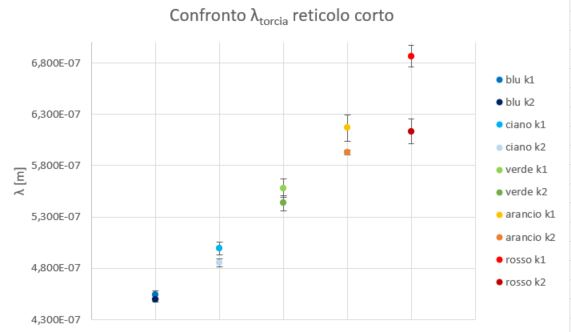
\includegraphics[width=0.6\linewidth]{TorciaCorto_graph.JPG}
    \caption{Grafico di confronto di lunghezze d'onda ottenute al primo e al secondo ordine}
    \label{confrontoCorto}
\end{figure}

Appare evidente sia dai dati riportati nelle tabelle sopra che dalla Figura \ref{confrontoCorto} che al crescere della lunghezza d'onda aumenti la discrepanza tra due righe dello stesso colore al primo e al secondo ordine. Ritengo che anche questo sia spiegabile alla luce del fatto che il secondo ordine di massimo abbia maggiore dispersione angolare, e quindi maggiore difficoltà nel misurare con precisione uno stesso punto. Questo si nota soprattutto nel verde e nel rosso, che, oltre a essere alcune delle più discrepanti (il rosso ha una discrepanza di $4,51\sigma$ tra i due ordini), sono al secondo ordine le più incerte. Inoltre il ciano e l'arancione non appaiono nello spettro per $m=2$ di destra, e questo inevitabilmente porta le misure ad avere una componente sistematica che aumenta il loro valore.

\vspace{3mm}

Pertanto ritengo che alla luce di queste considerazioni si possa non considerare attendibile la misura raccolta al secondo ordine e tenere per un confronto con quanto ottenuto nel reticolo lungo (prossima sezione) solo l'ordine 1.

\pagebreak
\subsection{Reticolo lungo}

Come già descritto nelle sezioni precedenti si è provveduto a sostituire il reticolo e a fare tutte le verifiche necessarie per iniziare la misura in condizioni ottimali. Sfortunatamente il tomo che sorreggeva lo smartphone è stato probabilmente perturbato durante lo scatto delle foto, il che ha portato ad una misura pesantemente affetta da gravi errori di ortogonalizzazione. 

\vspace{3mm}

Per completezza vengono riportati i dati, le figure e alcune considerazioni circa questa misura.

\begin{table}[h]
    \centering
        \begin{tabular}{||c|c|c||}
            \hline
            \# & $z [m]$ & $\sigma_z [m]$\\
            \hline
            1 & 4,43 & 0,01 \\
            2 & 4,44 & 0,01 \\
            3 & 4,42 & 0,01 \\
            4 & 4,43 & 0,01 \\
            5 & 4,45 & 0,01 \\
            6 & 4,43 & 0,01 \\
            7 & 4,43 & 0,01 \\
            \hline
            $z_{best}$ & 4,43 & 0,01 \\
            \hline
        \end{tabular}
    \caption{Misura di $z$}
\end{table}

\begin{figure}[h]
    \centering
    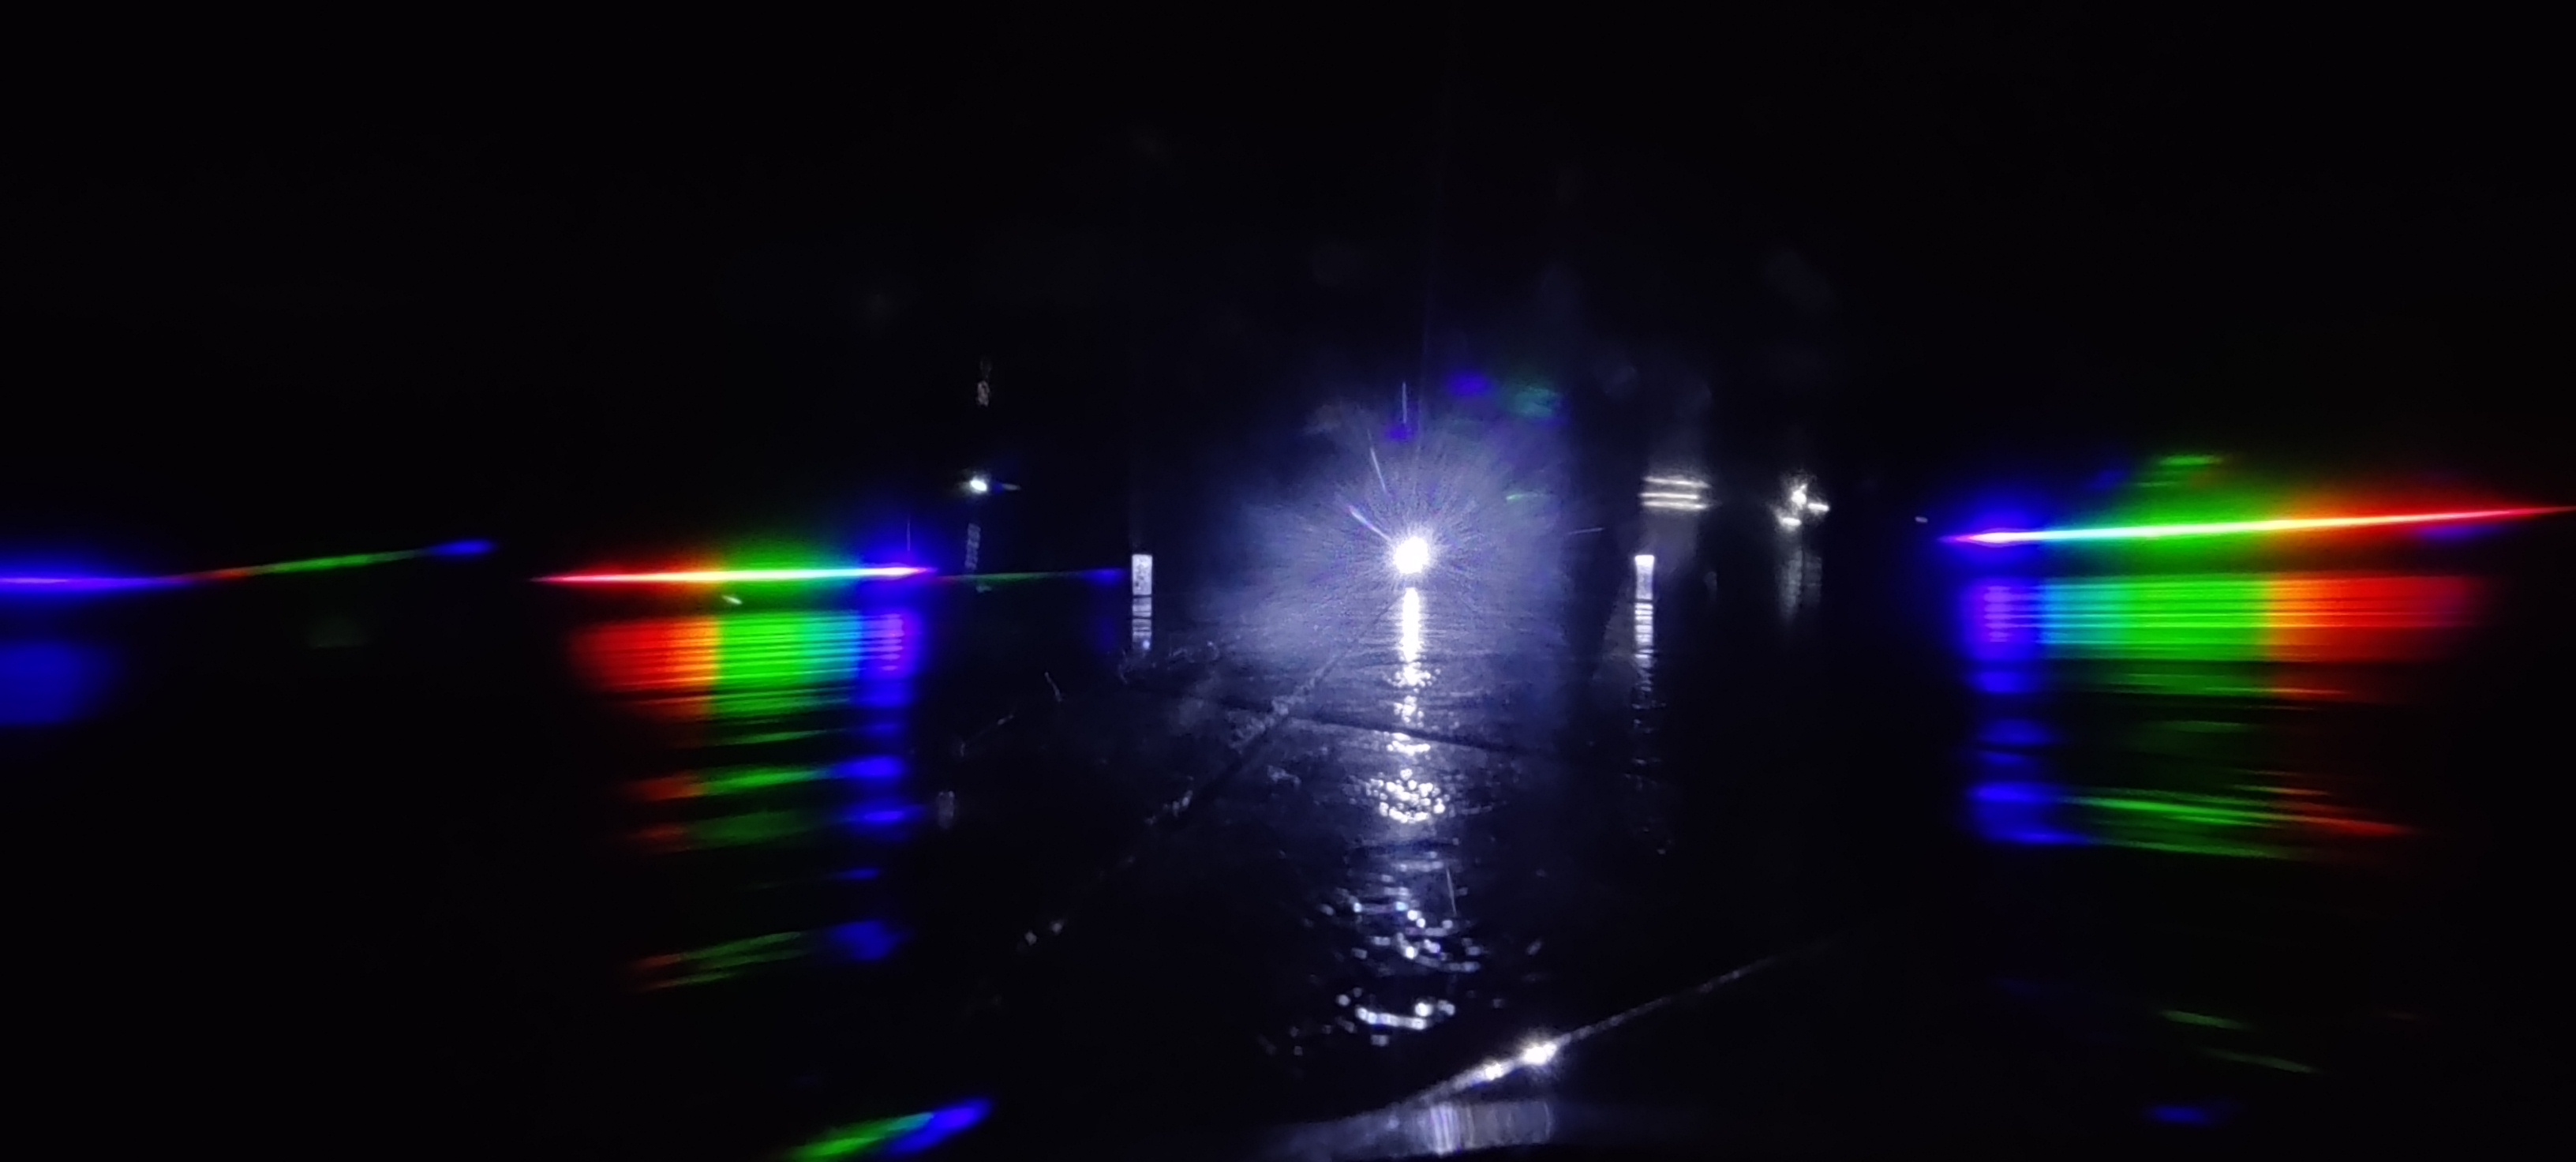
\includegraphics[width=0.7\linewidth]{TorciaLungo1_OFF.jpg}
    \caption{Diffrazione della torcia su reticolo lungo. Si nota come lo spago non sia perpendicolare al piano della fotografia e come il secondo ordine di sinistra non sia allineato col primo.}
    \label{TorciaLungo}
\end{figure}

\begin{table}[h]
    \centering
    \begin{tabular}{||c|c|c|c|c|c||}
        \hline
        \# & \cellcolor{blue}$\Delta x_{blu}$ [m] & \cellcolor{cyan}$\Delta x_{ciano}[m]$ & \cellcolor{green}$\Delta x_{verde}[m]$ & \cellcolor{orange}$\Delta x_{arancio}[m]$ & \cellcolor{red}$\Delta x_{rosso}[m]$ \\
        \hline
        1 & 2,071 & 2,292 & 2,543 & 2,887 & 3,185 \\
        2 & 2,049 & 2,287 & 2,538 & 2,835 & 3,199 \\
        3 & 2,046 & 2,284 & 2,569 & 2,873 & 3,219 \\
        \hline
    \end{tabular}
    \caption{Misura del primo ordine a sinistra}
\centering
\begin{tabular}{||c|c|c|c|c|c||}
    \hline
    \# & \cellcolor{blue}$\Delta x_{blu}$ [m] & \cellcolor{cyan}$\Delta x_{ciano}[m]$ & \cellcolor{green}$\Delta x_{verde}[m]$ & \cellcolor{orange}$\Delta x_{arancio}[m]$ & \cellcolor{red}$\Delta x_{rosso}[m]$ \\
    \hline
    1 & 2,323 & 2,649 & 3,042 & 3,594 & 4,058 \\
    2 & 2,310 & 2,624 & 3,000 & 3,552 & 3,974 \\
    3 & 2,319 & 2,632 & 3,021 & 3,564 & 4,050 \\
    \hline
\end{tabular}
\caption{Misura del primo ordine a destra}
\end{table}

\begin{table}[h]
    \centering
\begin{tabular}{||c|c|c|c|c|c||}
    \hline
     & \cellcolor{blue}$\overline{\Delta x_{blu}}$ [m] & \cellcolor{cyan}$\overline{\Delta x_{ciano}} [m]$ & \cellcolor{green}$\overline{\Delta x_{verde}}[m]$ & \cellcolor{orange}$\overline{\Delta x_{arancio}}[m]$ & \cellcolor{red}$\overline{\Delta x_{rosso}}[m]$ \\
    \hline
    Media & 2,186 & 2,461 & 2,786 & 3,218 & 3,614 \\
    $\sigma$ & 0,131 & 0,174 & 0,236 & 0,353 & 0,414 \\
    \hline
\end{tabular}
\caption{$\Delta x$ medi per diffrazione della torcia sul reticolo lungo}
\end{table}

\begin{table}[h]
    \centering
\begin{tabular}{||c|c|c|c|c|c||}
    \hline
     $m = 1$ & \cellcolor{blue}$\lambda_{blu}$ [nm] & \cellcolor{cyan}$\lambda_{ciano} [nm]$ & \cellcolor{green}$\lambda_{verde}[nm]$ & \cellcolor{orange}$\lambda_{arancio}[nm]$ & \cellcolor{red}$\lambda_{rosso}[nm]$ \\
    \hline
    Media & 410,4 & 462,1 & 522,9 & 604,0 & 678,5 \\
    $\sigma$ & 30,2 & 38,2 & 49,6 & 71,4 & 83,0\\
    \hline
\end{tabular}
\caption{$\lambda$ per diffrazione della torcia sul reticolo lungo}
\end{table}

\clearpage
Procedendo a un confronto tra le misure dello spettro del primo ordine per la torcia, effettuate col reticolo corto, e del primo ordine effettuate col reticolo lungo si ottiene con poca sorpresa che all'aumentare della lunghezza d'onda diminuisce la distanza in deviazioni standard. Infatti le misure del reticolo lungo hanno incertezza crescente in maniera vertiginosa all'aumentare della lunghezza d'onda, il che garantisce la compatibilità (Tabella 26, Figura \ref{confrontotraidue}).

\begin{table}[h]
    \centering
\begin{tabular}{||c|c|c|c|c|c||}
    \hline
     $\sigma$ di differenza & \cellcolor{blue}blu& \cellcolor{cyan}ciano  & \cellcolor{green}verde & \cellcolor{orange}arancio & \cellcolor{red}rosso \\
    \hline
    Media & 1,43 & 0,97 & 0,70 & 0,18 & 0,10 \\
    \hline
\end{tabular}
\caption{Deviazioni standard di differenza tra lunghezze d'onda misurate al primo ordine con entrambi i reticoli}
\end{table}

\begin{figure}
    \centering
    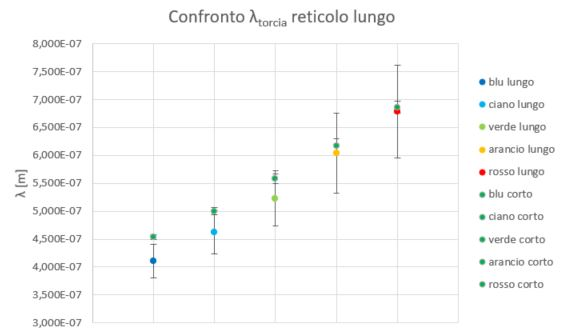
\includegraphics[width=0.6\linewidth]{Confronto_graph.JPG}
    \caption{Confronto grafico delle lunghezze d'onda della torcia ottenute con i due reticoli. La serie verde sono le misure del reticolo corto e sono verticalmente accoppiate col colore a cui si riferiscono}
    \label{confrontotraidue}
\end{figure}

%%% CONCLUSIONI %%%
\section{Conclusioni}

L'esperimento può dirsi concluso in maniera parzialmente soddisfacente.

\vspace{3mm}

La densità di fenditure del reticolo ignoto è stata stimata in $\rho_{lungo} = 1202 \pm 51 \; fend/mm$, con analogo ordine di grandezza del valore ottenuto da altri studenti (e che rende plausibile la misura solo nel caso in cui gli studenti abbiano ricevuto lo stesso reticolo di passo ignoto). 

\vspace{3mm}

I valori di $\lambda$ del puntatore ottenuti misurando con il reticolo corto risultano accettabili in quanto tengono conto della tecnologia RGB dei led ma comprendono anche alcune lunghezze d'onda frutto dell'unione dei tre colori base.

\vspace{3mm}

Sfortunatamente non è stato possibile confermare sperimentalmente la correttezza di $\rho_{lungo}$ a causa delle problematiche esposte in Sezione 4.2, che non hanno reso possibile un cofronto tra le lunghezze d'onda ricavate con i due reticoli. Ciononostante le misure delle lunghezze d'onda emesse dalla torcia diffratte dal reticolo corto sono attendibili come posizione nell'intervallo della luce visibile.



\end{document}